% v2-acmsmall-sample.tex, dated March 6 2012
% This is a sample file for ACM small trim journals
%
% Compilation using 'acmsmall.cls' - version 1.3 (March 2012), Aptara Inc.
% (c) 2010 Association for Computing Machinery (ACM)
%
% Questions/Suggestions/Feedback should be addressed to => "acmtexsupport@aptaracorp.com".
% Users can also go through the FAQs available on the journal's submission webpage.
%
% Steps to compile: latex, bibtex, latex latex
%
% For tracking purposes => this is v1.3 - March 2012

\documentclass[prodmode,acmtecs]{acmsmall} % Aptara syntax

\usepackage{amsmath}
\usepackage{dsfont}
\usepackage{mathtools}
\everymath{\displaystyle}

\usepackage{verbatim}
\usepackage{xspace}
\newcommand{\C}{\emph{C}\xspace}
\newcommand{\VM}{\emph{VM}\xspace}
\newcommand{\CEU}{\textsc{C\'{e}u}\xspace}
\newcommand{\code}[1] {{\small{\texttt{#1}}}}
\newcommand{\ax}{\code{[a]}\xspace}
\newcommand{\bx}{\code{[b]}\xspace}
\newcommand{\cx}{\code{[c]}\xspace}
\newcommand{\MM}[1] {\textcircled{\tiny{\textsf{#1}}}}

\newcommand{\ST}{\1\xrightarrow[~n~]{}\1}
\newcommand{\BT}{\xRightarrow[(i,E)]{}}
\newcommand{\LL}{\langle}
\newcommand{\RR}{\rangle}
\newcommand{\DS}{\displaystyle}
\newcommand{\rr}[1] {{\textbf{\scriptsize{#1}}}}

\newcommand{\1}{\;}
\newcommand{\2}{\;\;}
\newcommand{\3}{\;\;\;}
\newcommand{\5}{\;\;\;\;\;}
\newcommand{\ten}{\5\5}
\newcommand{\twenty}{\ten\ten}

\usepackage{color}
\definecolor{light}{gray}{0.97}
\definecolor{dark}{gray}{0.30}
%\definecolor{light}{rgb}{.90,.90,.90}
\definecolor{darkgreen}{rgb}{0,.50,0}
\definecolor{darkblue}{rgb}{0,0,.50}
\definecolor{darkred}{rgb}{.50,0,0}
\definecolor{darkpur}{rgb}{.50,0,.50}

\usepackage{listings}
%\usepackage{textcomp}
\usepackage{url}
\lstset{
%columns=fullflexible,
%basicstyle=\ttfamily,
escapeinside={||},
    %mathescape=true,
    language=C, % choose the language of the code
    basicstyle=\fontfamily{pcr}\selectfont\scriptsize\color{black},
    keywordstyle=\color{black}\bfseries, % style for keywords
    numbers=none, % where to put the line-numbers
    numberstyle=\tiny, % the size of the fonts that are used for the line-numbers
    backgroundcolor=\color{light},
    showspaces=false, % show spaces adding particular underscores
    showstringspaces=false, % underline spaces within strings
    showtabs=false, % show tabs within strings adding particular underscores
    %frame=single, % adds a frame around the code
    tabsize=2, % sets default tabsize to 2 spaces
    %rulesepcolor=\color{gray}
    captionpos=b, % sets the caption-position to bottom
    breaklines=false, % sets automatic line breaking
    %breakatwhitespace=false,
    numbersep=2em,
    % C was used in the blocksworld example to refer to block C and nowhere else
    emph={par,or,hor,do,end,loop,await,emit,input,event,call,with,%
          var,and,then,else,return,pure,deterministic,nohold,finalize,%
          class, every, FOREVER, this, spawn, in, pool, watching, until, 
          interface, each, abort, when, signal, PROC, CHAN, SIGNAL, PAR, not,
          bool, data, tag, escape, new, traverse,implementation,output,
          native,@const,@pure,@safe,define},
    emphstyle={\bfseries},
    commentstyle=\color{dark}\scriptsize,
    %xleftmargin=20pt,
    %xrightmargin=20pt,
    framesep=20pt,
    %upquote=true,
    %aboveskip={1.5\baselineskip},
}

% Metadata Information
%\acmVolume{9}
%\acmNumber{4}
%\acmArticle{39}
%\acmYear{2010}
%\acmMonth{3}

% Copyright
%\setcopyright{acmcopyright}
%\setcopyright{acmlicensed}
%\setcopyright{rightsretained}
%\setcopyright{usgov}
%\setcopyright{usgovmixed}
%\setcopyright{cagov}
%\setcopyright{cagovmixed}

% DOI
%\doi{0000001.0000001}

%ISSN
%\issn{1234-56789}

% Document starts
\begin{document}

% Page heads
%\markboth{G. Zhou et al.}{A Multifrequency MAC Specially Designed for WSN 
%Applications}

% Title portion
\title{The Design and Implementation of the Synchronous Language \CEU}

\author{
Francisco Sant'Anna
\affil{Departamento de Inform\'atica e Ci\^encia da Computa\c{c}\~ao, UERJ}
Roberto Ierusalimschy
\affil{Departamento de Inform\'atica, PUC--Rio}
Noemi Rodriguez
\affil{Departamento de Inform\'atica, PUC--Rio}
Silvana Rossetto
\affil{Departamento de Ci\^encia da Computa\c{c}\~ao, UFRJ}
Adriano Branco
\affil{Departamento de Inform\'atica, PUC--Rio}
}

% NOTE! Affiliations placed here should be for the institution where the
%       BULK of the research was done. If the author has gone to a new
%       institution, before publication, the (above) affiliation should NOT be changed.
%       The authors 'current' address may be given in the "Author's addresses:" block (below).
%       So for example, Mr. Abdelzaher, the bulk of the research was done at UIUC, and he is
%       currently affiliated with NASA.

\begin{abstract}
\CEU is a synchronous language targeting soft real-time systems.
It is inspired by Esterel and has a simple semantics with fine-grained control
over program execution.
%
\CEU uses an event-triggered notion of time that enables compile-time checks to 
detect conflicting concurrent statements, resulting in deterministic and 
concurrency-safe programs.
%
We present the particularities of our design in comparison to Esterel, such as 
stack-based internal events, concurrency checks, safe integration with \C, 
and first-class timers.
%
We also present two implementation back ends:
one aiming for resource efficiency and interoperability with \C,
and another as a virtual machine that allows remote reprogramming.
\end{abstract}

%
% The code below should be generated by the tool at
% http://dl.acm.org/ccs.cfm
% Please copy and paste the code instead of the example below. 
%
%\begin{CCSXML}
%<ccs2012>
 %<concept>
  %<concept_id>10010520.10010553.10010562</concept_id>
  %<concept_desc>Computer systems organization~Embedded systems</concept_desc>
  %<concept_significance>500</concept_significance>
 %</concept>
 %<concept>
  %<concept_id>10010520.10010575.10010755</concept_id>
  %<concept_desc>Computer systems organization~Redundancy</concept_desc>
  %<concept_significance>300</concept_significance>
 %</concept>
 %<concept>
  %<concept_id>10010520.10010553.10010554</concept_id>
  %<concept_desc>Computer systems organization~Robotics</concept_desc>
  %<concept_significance>100</concept_significance>
 %</concept>
 %<concept>
  %<concept_id>10003033.10003083.10003095</concept_id>
  %<concept_desc>Networks~Network reliability</concept_desc>
  %<concept_significance>100</concept_significance>
 %</concept>
%</ccs2012>
%\end{CCSXML}

%\ccsdesc[500]{Computer systems organization~Embedded systems}
%\ccsdesc[300]{Computer systems organization~Redundancy}
%\ccsdesc{Computer systems organization~Robotics}
%\ccsdesc[100]{Networks~Network reliability}

%
% End generated code
%

% We no longer use \terms command
%\terms{Design, Algorithms, Performance}

\keywords{
Concurrency, Determinism, Embedded Systems,
Esterel, Synchronous, Reactivity
}

%\acmformat{Gang Zhou, Yafeng Wu, Ting Yan, Tian He, Chengdu Huang, John A.  
%Stankovic,
%and Tarek F. Abdelzaher, 2010. A multifrequency MAC specially
%designed for  wireless sensor network applications.}
% At a minimum you need to supply the author names, year and a title.
% IMPORTANT:
% Full first names whenever they are known, surname last, followed by a period.
% In the case of two authors, 'and' is placed between them.
% In the case of three or more authors, the serial comma is used, that is, all author names
% except the last one but including the penultimate author's name are followed by a comma,
% and then 'and' is placed before the final author's name.
% If only first and middle initials are known, then each initial
% is followed by a period and they are separated by a space.
% The remaining information (journal title, volume, article number, date, etc.) is 'auto-generated'.

%\begin{bottomstuff}
%This work is supported by the National Science Foundation, under
%grant CNS-0435060, grant CCR-0325197 and grant EN-CS-0329609.

%Author's addresses: G. Zhou, Computer Science Department,
%College of William and Mary; Y. Wu  {and} J. A. Stankovic,
%Computer Science Department, University of Virginia; T. Yan,
%Eaton Innovation Center; T. He, Computer Science Department,
%University of Minnesota; C. Huang, Google; T. F. Abdelzaher,
%(Current address) NASA Ames Research Center, Moffett Field, California 94035.
%\end{bottomstuff}

\maketitle

\section{Introduction}

An established alternative to \C in the field of embedded systems is the family 
of reactive synchronous languages \cite{rp.twelve}.
%
Two major styles of synchronous languages have evolved:
in the \emph{control}--\emph{imperative} style, programs are structured with 
control flow primitives, such as parallelism, repetition, and preemption;
in the \emph{dataflow}--\emph{declarative} style, programs can be seen as 
graphs of values, in which a change to a value is propagated through its 
dependencies without explicit programming.
%
Of the control-based languages, Esterel~\cite{esterel.ieee91} was the 
first to appear and succeed, influencing a number of embedded languages, such 
as \emph{Reactive-C}~\cite{rp.rc}, \emph{OSM}~\cite{wsn.osm}, 
\emph{Sync-C}~\cite{rp.synchc}, and \emph{PRET-C}~\cite{rp.pretc}.

% TODO-no: SCCharts?, SynchCharts?

Despite its success and influence, Esterel has a complex semantics that
requires careful static analysis to detect and refuse programs with 
\emph{causality} and \emph{schizophrenia} problems%
%These problems have an extensive coverage in the literature 
~\cite{esterel.constructive,esterel.d7,esterel.d6,esterel.d3,esterel.d5,esterel.d8,esterel.d1,esterel.schizo2}.
%
A complex semantics not only challenges the analysis and compilation of 
programs, but also affects the programmer's understanding about the code, who,
ultimately, has to solve the errors when facing corner cases.
%
Furthermore, Esterel's semantics is non-deterministic for intra-reaction
statements, which prevents threads from interacting with stateful system calls
safely and makes shared-memory concurrency not as straightforward as reading
and writing to shared variables.
%
%For instance, although Esterel supports orthogonal abortion of 
%threads~\cite{esterel.preemption}, it doesn't offer an effective mechanism to 
%release resources in use.

In this work, we present \CEU, a new programming language that inherits the 
synchronous and imperative mindset of Esterel but diverges in some fundamental 
semantic aspects.
%
\CEU proposes a semantics for soft real-time systems with fine-grained control
for intra-reaction execution which is amenable to concurrency checks that
improve safety.
%
The list that follows summarizes the contributions behind the design of \CEU:
%
\begin{itemize}
%
\item Unique and queue-based external events, which define the notion of time 
in \CEU.
% (Section~\ref{sec.ceu.exts}).
%
\item Stack-based internal events for intra-reaction communication, which also
provides a limited form of coroutines.
% (Section~\ref{sec.ceu.ints}).
%
\item Static concurrency checks to detect suspicious concurrent statements.
%(Section~\ref{sec.ceu.checks}).
%
\item Safe integration with \C that enforces finalization for external 
resources.
% (Section~\ref{sec.ceu.c}).
%
\item First-class timers with dedicated syntax and automatic synchronization.
%(Section~\ref{sec.ceu.timers}).
\end{itemize}
%
We also present a lightweight single-threaded implementation of \CEU with two 
back ends:
one aiming for resource efficiency and interoperability with \C,
and another as a virtual machine that allows remote reprogramming.
%
Our implementations target resource-constrained devices, such as \emph{Arduino} 
and \emph{MICAz} sensor nodes based on 8-bit microcontrollers%
\footnote{
Both \emph{Arduino} and \emph{MICAz} use the 8-bit \emph{ATmega328} 
microcontroller with 32K of FLASH and 2K of SRAM.
}, showing a practical aspect of the proposed semantics.
%:\url{http://www.atmel.com/devices/atmega328.aspx}}

In previous work~\cite{ceu.sensys13,ceu.terra}, we employed \CEU in the context 
of wireless sensor networks, developing a number of applications, protocols, 
and device drivers.
%
We evaluated the expressiveness of \CEU in comparison to event-driven code in 
\C and attested a reduction in source code size (around 25\%) with a small 
increase in memory usage (around 5--10\% for \emph{text} and 
\emph{data})~\cite{ceu.sensys13}.
%
For the \VM back end, applications have a bytecode footprint in the order of 
hundreds of bytes and can be transmitted over the air in a few 
packets~\cite{ceu.terra}.

The semantics of \CEU implies an implementation with a runtime stack and a
sequential scheduler.
In contrast with Esterel's semantics, this prevents programs to be compiled
directly and efficiently to hardware~\cite{esterel.constructive}.
It also makes difficult to statically determine worst-case reaction times
towards hard real-time systems~\cite{esterel.fixed}.

The rest of the paper is organized as follows:
Section~\ref{sec.ceu} discusses the design of \CEU, focusing on the fundamental 
differences to Esterel.
%Section~\ref{sec.sem} presents a formal semantics for the control primitives 
%of \CEU.
Section~\ref{sec.impl} presents the \C and \VM implementation back ends.
Section~\ref{sec.related} discusses other synchronous languages targeting 
embedded systems.
Section~\ref{sec.conclusion} concludes the paper.

%\begin{itemize}
        %\item Estendendo para outros dominios? (jogos, artigo Mod'15)
        %\item Usos: sala de aula, GSoC
%\item Semantica e Implementacao (nesse artigo, somente subset estatico)
% Artigo de Rust, nao resolve os problemas
%https://blog.skcript.com/asynchronous-io-in-rust-36b623e7b965
%state machines everywhere
%\end{itemize}

%Our work focuses on \emph{concurrency safety}, rather than \emph{type 
%safety}~\cite{wsn.safety}.%
%\footnote{
%We consider both safety aspects to be complimentary and orthogonal, i.e., 
%type-safety techniques could also be applied to \CEU.
%}

%As a trade-off, our design imposes limitations on the language expressiveness, 
%such as doing computationally-intensive operations and meeting hard real-time 
%responsiveness.

\section{The Design of \CEU}
\label{sec.ceu}

\CEU is a synchronous reactive language inspired by Esterel in which programs 
advance in a sequence of discrete reactions to external events.
%
%Regarding the similarities with Esterel,
%\CEU has a strong imperative flavor, with explicit control flow through 
%sequences, loops, and parallel compositions.
%
Like Esterel, \CEU is designed for control-intensive applications, supporting 
concurrent lines of execution, known as \emph{trails}, and broadcast 
communication through events.
%
Internal computations within a reaction (e.g. expressions, assignments, and 
system calls) are considered to take no time in accordance with the synchronous 
hypothesis~\cite{rp.hypothesis}.
An \code{await} is the only statement that halts a running reaction and allows 
a program to advance in this discrete notion of time.
%
To ensure that reactions run in bounded time and programs always progress, 
loops are statically required to contain at least one \code{await} statement in 
all possible paths~\cite{ceu.sensys13,esterel.primer}.
%
\CEU shares the same limitations with (core) Esterel and synchronous languages 
in general~\cite{esterel.preemption}:
computations that run in unbounded time (e.g., cryptography, image processing) 
do not fit the zero-delay hypothesis, and cannot be directly implemented.

Figure~\ref{lst.abro} illustrates the syntactic similarities between the 
languages, showing side-by-side the implementations in Esterel \ax and \CEU \bx 
for the following control specification:
%
\emph{``Emit an output O as soon as inputs A and B occur.
Reset this behavior each time input R occurs''}~\cite{esterel.primer}.
%
The first phrase of the specification, awaiting and emitting the events, is 
translated almost identically in the two languages (ln. 5--10, in both 
implementations), as Esterel's `$\|$' and \CEU's \code{par/and} constructs are 
equivalent.
%
For the second phrase, the reset behavior, the Esterel version uses an 
\code{abort-when} statement (ln. 4--11) which, in this case, serves the same 
purpose as \CEU's \code{par/or} (ln. 4--13):
the occurrence of event \code{R} aborts the awaiting statements in parallel and 
restarts the enclosing \code{loop}.

\begin{figure}
\begin{minipage}[t]{0.48\linewidth}
\begin{lstlisting}[numbers=left,xleftmargin=3.5em,mathescape=true]
input  A, B;
output O;
loop
   abort
      [
         await A
      $\|$
         await B
      ];
      emit O
   when R
end

.
\end{lstlisting}
\centering\small{\ax Esterel}
\end{minipage}
%
\begin{minipage}[t]{0.48\linewidth}
\begin{lstlisting}[numbers=left,xleftmargin=3.5em]
input  void A, B;
output void O;
loop do
   par/or do
      par/and do
         await A;
      with
         await B;
      end
      emit O;
   with
      await R;
   end
end
\end{lstlisting}
\centering\small{\bx \CEU}
\end{minipage}
%\rule{8.4cm}{0.37pt}
\caption{ A control specification implemented in Esterel and \CEU:
\emph{``Emit \code{O} after \code{A} and \code{B}, resetting each \code{R}.''}
A \code{par/and} terminates when both trails in parallel terminate.
A \code{par/or}  terminates when any trail terminates, aborting the 
other.
\label{lst.abro}
}
\end{figure}

% TODO-no: par/or vs abort, strong/weak abortion

Figure~\ref{lst.syn} shows the subset of the concrete syntax of \CEU used in
this paper as a quick reference.
%
In a separate document, we present the formal semantics with a simplified
abstract syntax~\cite{ceu.phd}.

\begin{figure}
\begin{lstlisting}
// DECLARATIONS

input  <type> <ids>;                        // external input  events
output <type> <ids>;                        // external output events
event  <type> <ids>;                        // internal events
var    <type> <id> = <exp>;                 // a variable with an initial value

// EVENT HANDLING

<id> = await <id>;                          // await an event and assign the received value
<id> = await <time>;                        // await time and assign the delayed delta
emit <id> => <exp>;                         // emit an event passing a value

// CONTROL FLOW

<stmt> ; <stmt>                             // sequence
if <exp> then <stmts> else <stmts> end      // conditional
loop do <stmts> end                         // repetition
do <stmts> end                              // explicit block

par/or  do <stmts> with <stmts> end         // aborts when one side terminates
par/and do <stmts> with <stmts> end         // terminates when both sides terminate
par     do <stmts> with <stmts> end         // never terminates

finalize <stmts> with <stmts> end           // block finalization

// INTEGRATION WITH C

<_id>(<exps>)                               // C call (identifier starts with `_')
native do <stmts> end                       // declarations in C
native @const <_ids>                        // annotations: constant symbols
native @pure  <_ids>                        //              pure functions
native @safe  <_ids> with <_ids>            //              non-conflicting symbols
\end{lstlisting}
\caption{ Subset of the concrete syntax of \CEU used in this paper.
\label{lst.syn}
}
\end{figure}

In the subsections that follow, we discuss the main differences between \CEU and
Esterel:
%
Unique and queue-based external events
    (\ref{sec.ceu.exts});
Stack-based internal events
    (\ref{sec.ceu.ints});
Static concurrency checks
    (\ref{sec.ceu.checks});
Safe integration with \C
    (\ref{sec.ceu.c});
and
First-class synchronized timers
    (\ref{sec.ceu.timers}).
We finish the section with a summary of our design
    (\ref{sec.ceu.summary}).

\subsection{ Unique and Queue-Based External Events }
\label{sec.ceu.exts}

Esterel defines time as a discrete sequence of logical unit instants or 
``ticks''.
At each tick, the program reacts to an arbitrary number of simultaneous input 
events from the environment.
In contrast, \CEU defines time as a discrete sequence of reactions to
unique input events.
At each input event, which constitutes a logical unit of time, the program 
reacts exclusively to it.
The event-triggered execution of a program in \CEU is as 
follows~\cite{ceu.sensys13}:
%
\begin{enumerate}
\item The program initiates the ``boot reaction'' in a single trail (but 
      parallel constructs may create new trails).
\item Active trails execute until they await or terminate, one after the other.
      This step is named a \emph{reaction chain}, and always runs in bounded 
      time.
\item The program goes idle and the environment takes control.
\item On the occurrence of a new external input event, the environment awakes 
      \emph{all} trails awaiting that event.
      It then goes to step 2.
\end{enumerate}
%
A program must react to an event completely before handling the next 
one.
%
Based on the synchronous hypothesis, a program takes a negligible time on step 
2 and is always idle on step 3.
In practice, if a new external input event occurs while a reaction chain is 
running, it is enqueued to occur in a subsequent reaction.

\begin{figure}[!htb]
\centering
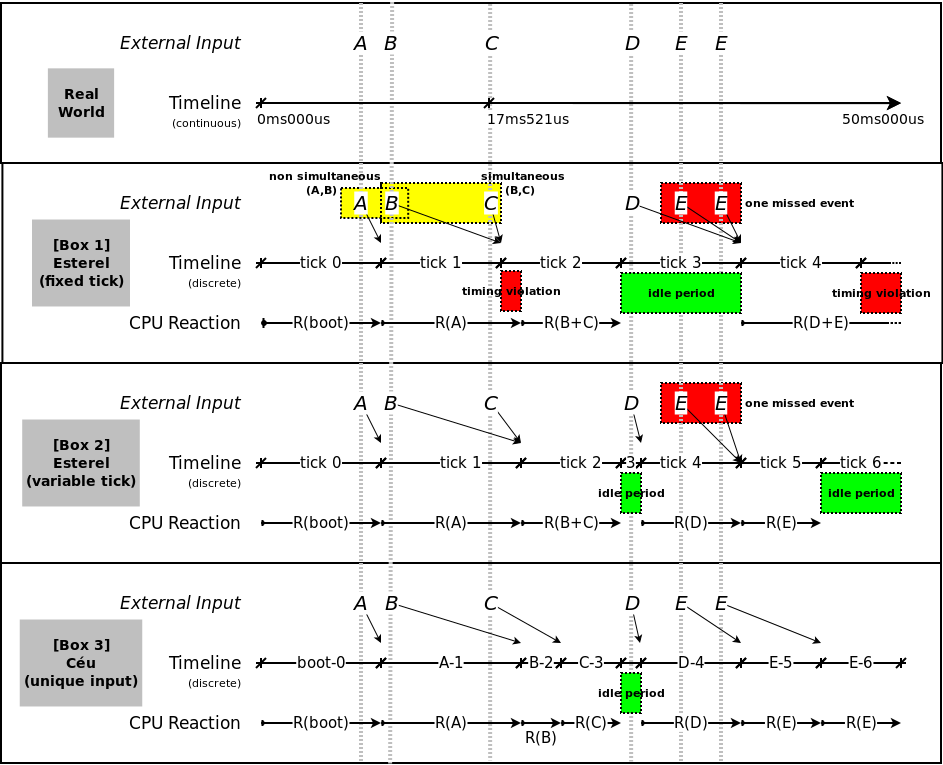
\includegraphics[width=\columnwidth]{tick}
\caption{The discrete notions of time in Esterel and \CEU.
\label{fig.ticks}
}
\end{figure}

Figure~\ref{fig.ticks} compares the discrete notions of time in two variations 
of Esterel and in \CEU.
The box \code{Real World} assumes an external observer with an absolute
reference clock which timestamps event occurrences over a
continuous timeline~\cite[Chapter~3]{es.time} (e.g., event \code{C} occurs at
$17ms521us$).
The other boxes show how the same occurring events fit differently in each 
logical notion of time.
%
\begin{itemize}
\item \code{[Box-1]}:
\emph{Esterel with fixed-length ticks}~\cite{esterel.fixed}.
%
(Usually referred as \emph{sample-driven execution}~\cite{rp.twelve}.)
%
We assume a reaction \code{R(boot)} at \code{tick-0} which happens before any 
input.
%
The input \code{A} ``physically'' occurs during the boot reaction but, because 
time is discrete, its corresponding reaction only executes in the next tick.
%
Note that \code{R(A)} takes more time than \code{tick-1} and invades 
\code{tick-2}, causing a \emph{timing violation}~\cite{esterel.fixed}.
%
The events \code{B} and \code{C} occur during \code{tick-1} and are delayed to 
happen \emph{simultaneously} at \code{tick-2} with \code{R(B+C)}.
%
Since no new events occur during \code{tick-2}, the CPU stays idle during the 
whole \code{tick-3}.
%
Finally, one instance of event \code{D} and two instances of event \code{E} 
occur during the idle \code{tick-3}.
However, only one occurrence of \code{E} can be considered in \code{R(D+E)}.
%
\item \code{[Box-2]}:
\emph{Esterel with variable-length ticks}~\cite{esterel.variable}.
This approach avoids the timing violation for \code{R(A)} and also results in
smaller idle periods because it adjusts the tick lengths to match the CPU times 
for the reactions.
For instance, the occurrence of \code{D} interrupts the idle \code{tick-3} to 
react alone as \code{R(D)} at \code{tick-4}.
Similarly to the fixed-tick approach, only one of the two simultaneous 
occurrences of \code{E} is considered at \code{tick-5}, now because \code{R(D)} 
takes too long.
%
\item \code{[Box-3]}:
\emph{\CEU with unique and queue-based input events}.
We also assume a reaction \code{R(boot)} before any input.
%
Because the occurrence of event \code{A} is unique during \code{R(boot)}, the 
behavior in \CEU is similar to \code{Box-2} for its first two reactions 
(\code{tick-0} and \code{tick-1}).
%
However, \CEU does not consider the events \code{B} and \code{C} as 
simultaneous, and handles each in subsequent reactions \code{R(B)} and 
\code{R(C)}.
%
We assume the CPU times for \code{R(B+C)} in Esterel and \code{R(B)+R(C)} in 
\CEU to be roughly the same.
This way, the first idle periods in \code{Box-2} and \code{Box-3} coincide.
%
Finally, \CEU reacts to the two instances of \code{E} independently, which are
handled in sequence.
%
%Note that, by definition, each reaction corresponds to an event occurrence of 
%the same length.
\end{itemize}

Sample-driven execution maps directly to hardware implementations and
involve no runtime queues.
%
However, considering the soft real-time application domain of \CEU, we
decided for the unique and queue-based semantics in \CEU for the reasons
that follow:
%
\begin{itemize}
\item \textbf{A ``tick'' is implementation dependent:}
Tick lengths are not part of the program specification.
For instance, if we log the \code{Real World} box timeline and reproduce it in
implementations with different tick lengths, the behaviors might diverge.
%
\item \textbf{Events are never absolutely simultaneous:}
We consider that the notion of simultaneity should be defined explicitly for
each use case (to be discussed in Section~\ref{sec.ceu.timers}).
%In Section~\ref{sec.ceu.timers}, after introducing internal events and 
%first-class timers, we show an example to illustrate how to detect simultaneous 
%button clicks in \CEU.
In tick-based approaches, simultaneity depends on the length of discrete ticks.
For instance, in \code{box-1} and \code{box-2} of Figure~\ref{fig.ticks}, 
events \code{B} and \code{C} are simultaneous, even though \code{A} and
\code{B} ``physically'' happen much closer to one another.
%
\item \textbf{Unique input events imply mutual exclusion:}
Reactions to exclusive events are atomic and never overlap.
Automatic mutual exclusion simplifies reasoning about concurrency and is a 
prerequisite for the concurrency checks to be discussed in 
Section~\ref{sec.ceu.checks}.
\end{itemize}

Note that Esterel supports declarations for mutually exclusive inputs that
cannot be simultaneous in the same reaction
(e.g., ``\code{relation A\#B\#C\#D\#E;}'')~\cite{esterel.primer}.
Making all inputs mutually exclusive and adopting the variable-length-tick
approach is equivalent to \CEU's notion of time, which can be seen as an
imposed restriction on the semantics of Esterel.

The synchronous hypothesis for \CEU holds if the reactions run faster than the 
rate of incoming input events.
Otherwise, the application continuously accumulates delays between the real 
occurrence and actual reaction of a given event (we discuss implementation
considerations in Sections~\ref{sec.impl.single}~and~\ref{sec.impl.environment}).
%
This is also the case for the variable-length-tick approach of Esterel, since 
the more inputs to handle, the longer the reaction takes, and the more inputs 
accumulate for subsequent ticks.
%
For the fixed-length-tick approach of Esterel, a breach in the synchronous 
hypothesis causes timing violations, requiring \emph{worst case reaction time} 
analysis to infer appropriate tick lengths~\cite{esterel.fixed}.
% TODO-no: Such analysis is orthogonal
%
For soft real-time systems, accumulating delays and occasionally postponing
reactions might be enough.
However, hard real-time systems require a more robust approach such as
determining fixed-length ticks that can be statically verified.

A limitation of event-triggered execution is that all program behavior is 
purely reactive, given that no code can execute in the absence of inputs.
%
Tick-triggered execution allows for active behavior, since code can execute 
regularly on every tick.
%
Although \CEU supports active \emph{asynchronous} execution~\cite{ceu.tr}, its 
synchronous core is still purely reactive.

\begin{comment}
> Multiclock Esterel
The Esterel synchronous reactive language [5,4,6], which we call Classic Esterel
in this paper, is based on a single-clock instantaneous interaction principle. The
behavior of a program is defined by a sequence of reactions to input sequences.
The execution environment decides when the program is provided an input, and
a reaction is viewed as the simultaneous production of an output response to
an input event. We call ticks the instants in which reactions occur, and master
clock the sequence of these instants (it is a logical clock and no time regularity
is required).

An Esterel Processor with Full Preemption Support and its Worst Case Reaction 
Time Analysis
3. ESTEREL AND THE KIEL ESTEREL PROCESSOR
The execution of an Esterel program is divided into (logical) instants, or 
(logical) ticks, which are conceptually executed infinitely fast.
An Esterel program interacts with its environment through signals, which are 
either present throughout a logical instant or absent.
Input signals are sampled at each tick, and each tick may generate output 
signals.
It would be possible to have the system just compute one logical instant after 
the other, to start with the next reaction as soon as the previous one has 
finished; however, typically the ticks are executed at some fixed frequency, 
resulting in an interval T between each tick, where T is determined by the 
real-time requirements of the system.
The conceptually infinitely fast computation of the reaction within a logical 
tick, plus in the case of Esterel the unique signal presence/absence status 
throughout a logical tick, together constitute the synchrony hypothesis. In 
practice, the results of a logical instant of course cannot be computed 
infinitely fast; however, to maintain the abstraction of the synchrony 
hypothesis, a logical instant must be computed within some desired reaction 
time T.

4. WORST CASE REACTION TIME ANALYSIS
TODO-no: requires this, what about this in the context of MThreads??
Towards Direct Execution of Esterel Programs on Reactive Processors
3.1 Preserving the Synchrony Hypothesis
The synchronous model implies that reactions to input signals are instantaneous 
and occur at discrete logical instants called ticks.
As a result, a sequence of actions may need to be performed within the duration 
of a single tick.
In order to model the logical tick of Esterel in RePIC, a tick with variable 
length in terms of absolute time is implemented.
The duration of one tick is determined by the time required to execute all the 
instantaneous instructions that are placed between any two consecutive await 
(i.e. TAWAIT, SAWAIT or CAWAIT) or halt instructions which are the tick 
delimiting instructions.
(TODO-no: tem figuras)
\end{comment}

\subsection{ Stack-Based Internal Events }
\label{sec.ceu.ints}

In Esterel, the behavior of internal and external signals is equivalent.
%In particular, programs can emit external and internal signals simultaneously, 
%with all coexisting during the entire reaction.
%
%In \CEU, a reaction starts from an external input event and programs cannot 
%emit inputs at all.
%Therefore, the occurring input event is unique during the entire reaction, 
%resulting in intrinsic queue-based handling.
%
%In \CEU, subsequent external events coming from the environment define a 
%timeline, which programs cannot interfere by emitting new external events.
%
%To cope with deterministic intra-reaction communication, \CEU supports 
%internal events which programs can \code{emit} and \code{await}.
In \CEU, in contrast with queue-based external events, internal events follow a 
stack-based execution policy similar to subroutine calls in typical programming 
languages.
%
Figure~\ref{lst.prints} illustrates the use of internal signals (events) in 
Esterel \ax and \CEU \bx.
%
In Esterel, when \code{A} occurs, the program emits \code{B} (ln.  4--5) and 
both events become active, resulting in the invocation of \code{f()} and 
\code{g()} in no particular order (ln. 6,9).
%
In \CEU, when \code{A} occurs, the program behaves as follows:
%
{\small
\begin{enumerate}
\setlength{\itemsep}{0pt}
\item 1st trail awakes, broadcasts \code{b}, and pauses (ln. 4--5).
\item 2nd trail awakes, calls \code{\_g()}, and terminates (ln. 8--9).
      \emph{(No other trails awake to \code{b}.)}
\item 1st trail (on top of the stack) resumes, calls \code{\_f()}, and 
    terminates (ln. 5--6).
\item Both trails have terminated, so the \code{par/and} rejoins, and the 
program also terminates.
\end{enumerate}
}

\begin{figure}
\begin{minipage}[t]{0.43\linewidth}
\begin{lstlisting}[numbers=left,xleftmargin=3.5em,mathescape=true]
input  A;   // external
signal B;   // internal
[[
    await A;
    emit B;
    call f();
$\|$
    await B;
    call g();
]]
\end{lstlisting}
\centering\small{\ax Esterel}
\end{minipage}
%
\begin{minipage}[t]{0.53\linewidth}
\begin{lstlisting}[numbers=left,xleftmargin=3.1em]
input void A;  // external (in uppercase)
event void b;  // internal (in lowercase)
par/and do
    await A;
    emit b;
    _f();
with
    await b;
    _g();
end
\end{lstlisting}
\centering\small{\bx \CEU}
\end{minipage}
%\rule{8.4cm}{0.37pt}
\caption{ Internal signals (events) in Esterel and \CEU: similar syntax, but 
different semantics.
\label{lst.prints}
}
\end{figure}

Internal events provide fine-grained execution control and can express a 
limited form of subroutines, as depicted in Figure~\ref{lst.sub}.
The ``subroutine'' \code{inc} is defined as a loop (ln. 3--6) that continuously 
awaits its identifying event (ln. 4), incrementing the value passed by
reference (ln. 5).
A trail in parallel (ln. 8--11) invokes the subroutine through an \code{emit 
inc} (ln. 10) in reaction to some code (ln. 9).
Given the stacked execution for internal events, the calling trail pauses, the 
subroutine awakes (ln. 4), runs its body (yielding \code{v=2}), loops, and 
awaits the next ``call'' (ln. 4, again).
Only after this sequence, the calling trail resumes and passes the assertion 
test (ln. 10--11).

\CEU also supports nested \code{emit} invocations for internal events.
For instance, the body of the subroutine \code{inc} in Figure~\ref{lst.sub} 
could \code{emit} another event after awaking (ln. 4), creating a new level in 
the stack.
The runtime stack constitutes fine-grained micro reactions, with one on top of 
the other, all inside the same reaction to an external event.
%Internal events provide a fine-grained intra-reaction control mechanism.

\begin{figure}
\begin{lstlisting}[numbers=left,xleftmargin=2em]
event int* inc; // subroutine `inc'
par/or do
    loop do     // definitions are loops
        var int* p = await inc;
        *p = *p + 1;
    end
with
    var int v = 1;
    <...>
    emit inc => &v; // call `inc'
    _assert(v==2);  // after return
end
\end{lstlisting}
\caption{ Subroutine \code{inc} is defined in a loop (ln. 3--6), in parallel 
with the caller (ln. 8--11).
\label{lst.sub}
}
\end{figure}

% TODO-no: .. will probably expect that duplicating the  emit inc => &v; line 
% would result in v==3.

On the one hand, this form of subroutine has a significant limitation that it 
cannot express recursive calls: an \code{emit} to itself is always ignored, 
given that a running body cannot be awaiting itself.
%
On the other hand, this very same limitation brings some important safety 
properties to subroutines:
first, they are guaranteed to react in bounded time;
second, memory for locals is also bounded, not requiring data stacks.
%
Also, this form of subroutine can use the other primitives of \CEU, such as 
parallel compositions and the \code{await} statement.
In particular, they await keeping context information such as locals and the 
program counter, similarly to coroutines~\cite{lua.coroutines}.
%
In previous work, we build other advanced control mechanisms on top of internal 
events, such as resumable exceptions and reactive variables~\cite{ceu.rem13}.
%In Section~\ref{sec.adv.excpt} we show how to use them to implement 
%exceptions.

Another distinction regarding event handling in comparison to \CEU is that 
Esterel supports same-cycle bi-directional 
communication~\cite{esterel.compiling}, i.e., two threads can react to one 
another during the same cycle due to mutual signal dependencies
(a.k.a. \emph{instantaneous dialogue}~\cite{rp.book}).
%
\CEU takes a different approach, posing a restriction that an \code{await} is
only valid for the next reaction, i.e., if an \code{await} and \code{emit}
occur simultaneously in parallel trails, the \code{await} does not awake.
%
These \emph{delayed awaits} avoid corner cases of instantaneous
termination and re-execution of statements in the same reaction (known as
\emph{schizophrenic statements}~\cite{esterel.constructive}).
%
Also, this approach does not require data dependency analysis like Esterel
(e.g., \emph{``(set or reset of a signal must always precede any test of this
signal (signal coherence law and constructivity)''}~\cite{esterel.saxort}).

\begin{figure}
\begin{lstlisting}[numbers=left,xleftmargin=2em]
event void e,f;
loop do
    par/or do
        await e;
    with
        emit e;     // w/o delayed awaits, the emit awakes 1st trail
        await f;    // and restarts the loop instantaneously
    end
end
\end{lstlisting}
\caption{ Delayed awaits prevents re-execution of statements by design.
\label{lst.await}
}
\end{figure}

The example in Figure~\ref{lst.await} illustrates delayed awaits, which 
prevents infinite execution in the loop.
Both sides of the \code{par/or} have an \code{await} statement (ln. 4,7), which 
characterizes the enclosing \code{loop} as non instantaneous (ln 2--9).
However, if the \code{emit e} (ln. 6) could awake the \code{await e} 
instantaneously (ln. 4), the \code{par/or} would terminate and restart the 
\code{loop} also instantaneously, resulting in infinite execution.
%
\begin{comment}
\begin{figure}
%\begin{minipage}[t]{0.50\linewidth}
\begin{lstlisting}[numbers=left,xleftmargin=3em]
event void e;
par do
    loop do
        <...>     // code that awaits some period
        emit e;   // periodic request
    end
with
    loop do
        <...>     // code to execute immediately and then periodically
        await e;  // await after
    end
end
\end{lstlisting}
%\end{minipage}
%
%\begin{minipage}[t]{0.50\linewidth}
%\begin{lstlisting}[numbers=left,xleftmargin=3em]
%event void e;
%var bool should_execute = false;
%par do
%    loop do
%        <...>         // code that awaits
%        if <...> then // some conditon
%            should_execute = true;
%            emit e;
%        end
%    end
%with
%    loop do
%        if should_execute then
%            <...>     // code to execute
%        end
%        await e;
%    end
%end
%\end{lstlisting}
%\end{minipage}
%
\caption{ An example that circumvents the \emph{delayed await} by post-fixing 
the \code{await} inside the \code{loop}.
% (in the left), and by copying the condition test (in the right).
\label{lst.delay}
}
\end{figure}
\end{comment}
%
In atypical scenarios requiring immediate awake, delayed awaits can be 
circumvented by placing the code to execute before the \code{await}.
%
\begin{comment}
For instance, sometimes we need to execute a block of code immediately, and 
then periodically from internal event requests, as illustrated in 
Figure~\ref{lst.delay}.
In this case, the \code{await} moved to the end of the loop (ln. 10) makes the 
periodic code to also execute immediately (ln. 9), and then in reactions to 
each \code{emit} request (ln. 5).
If the periodic \code{emit} depends on a condition, then the code 
transformation becomes more intricate, requiring an extra condition test around 
the periodic code to prevent its immediate execution.
\end{comment}
%
On the one hand, we transfer the burden of dealing with these corner cases to 
the programmer.
On the other hand, we simplify the semantics of the language and eliminate the 
need for complex analysis to deal with schizophrenic statements.

%\newpage %TTT

\subsection{ Static Concurrency Checks }
\label{sec.ceu.checks}

Embedded applications make extensive use of global memory and shared resources, 
such as through memory-mapped registers and system calls to device drivers.
Hence, an important goal of \CEU is to ensure a reliable behavior for programs 
with concurrent lines of execution sharing memory and interacting with the 
environment.

Esterel is only deterministic with respect to external behavior: \emph{``the
same sequence of inputs always produces the same sequence of 
outputs''}~\cite{esterel.primer}.
%
However, the execution order for operations within a reaction is 
non-deterministic: \emph{``if there is no control dependency, as in
\code{(call~f1()~||~call~f2())},
the order is unspecified and it would be an error to rely on 
it''}~\cite{esterel.primer}.
%
For this reason, Esterel, does not support shared-memory concurrency:
\emph{``if a variable is written by some thread, then it can neither be read
nor be written by concurrent threads''}~\cite{esterel.primer}.
%
A number of Esterel-inspired synchronous languages enforce an arbitrary 
execution order for statements in multiple lines of execution to achieve 
intra-reaction determinism
(%
\emph{Reactive C}~\cite{rp.rc},                 % 1991
\emph{Protothreads}~\cite{wsn.protothreads},    % 2006
\emph{SOL}~\cite{wsn.sol},                      % 2007
\emph{SC}~\cite{rp.synchc},                     % 2009
and
\emph{PRET-C}~\cite{rp.pretc}%                  % 2010
).
%, e.g., based on lexical order or manual priority assignment.
%
\CEU also takes the deterministic approach and, when multiple trails are active 
during the same reaction, they are scheduled in lexical order, i.e., in the 
order they appear in the program source code.

\begin{figure}
\begin{minipage}[t]{0.50\linewidth}
\begin{lstlisting}[numbers=left,xleftmargin=3em]
input void A, B;
var int x = 1;
par/and do
    await A;
    x = x + 1;
with
    await B;
    x = x * 2;
end
\end{lstlisting}
\centering\small{\ax Accesses to \code{x} are safe}
\end{minipage}
%
\begin{minipage}[t]{0.50\linewidth}
\begin{lstlisting}[numbers=left,xleftmargin=3em]
input void A;
var int y = 1;
par/and do
    await A;
    y = y + 1;
with
    await A;
    y = y * 2;
end
\end{lstlisting}
\centering\small{\bx Accesses to \code{y} are unsafe}
\end{minipage}
%\rule{8.4cm}{0.37pt}
\caption{ Shared-memory concurrency in \CEU:
example \ax is safe because the trails access \code{x} atomically in different 
reactions;
example \bx is unsafe because both trails access \code{y} in the same reaction.
\label{lst.shared}
}
\end{figure}

Even so, we consider that enforcing an arbitrary execution order can be 
misleading in some cases.
%
For instance, consider the two examples in Figure~\ref{lst.shared}, both 
defining a shared variable (ln. 2), and assigning to it in parallel trails (ln.  
5, 8).
%
In the example \ax, the two assignments to \code{x} can only execute in 
reactions to different events \code{A} and \code{B}, which cannot occur 
simultaneously by definition (Section~\ref{sec.ceu.exts}).
Hence, for the sequence \code{A->B}, \code{x} becomes \code{4} 
(\code{(1+1)*2}), while for \code{B->A}, \code{x} becomes \code{3} 
(\code{(1*2)+1}).
%
In the example \bx, the two assignments to \code{y} are simultaneous because 
they execute in reaction to the same event \code{A}.
Since \CEU employs lexical order for intra-reaction statements, the execution 
is still deterministic, and \code{y} always becomes \code{4} (\code{(1+1)*2}).
%
However, an (apparently innocuous) change in the order of trails modifies the 
semantics of the program, which we consider unsafe.

To mitigate this threat, \CEU performs concurrency checks at compile time to 
detect conflicting accesses to shared variables:
if a variable is written in a trail segment, then a concurrent trail segment 
cannot read or write to that variable, nor dereference a pointer of that 
variable type.
%An analogous policy is applied for pointers \emph{vs} variables and pointers 
%\emph{vs} pointers.
%
Concurrency in \CEU is characterized when two or more trail segments in 
parallel react to the same input event.
A trail segment is a sequence of statements followed by an \code{await} (or 
termination).
%
Considering the examples in Figure~\ref{lst.shared}:
%
\begin{itemize}
\item The assignments to \code{x} (\ax:2,5)
      \textbf{cannot} be concurrent because they are \textbf{not} in parallel trails.
\item The assignments to \code{x} (\ax:5,8)
      \textbf{cannot} be concurrent because they \textbf{cannot} execute during 
      the same reaction.
\item The assignments to \code{y} (\bx:5,8)
      \textbf{can} be concurrent because they are in parallel trails and 
      \textbf{can} execute during the same reaction.
\end{itemize}
%
The detection algorithm, which is depicted in Section~\ref{sec.impl.checks},
inspects all possible \code{await} statements that precede a variable access
and keeps a list with all corresponding awaking events.
Then, it checks all accesses in parallel trails to see if they share an awaking 
event.
If it is the case, the compiler warns about the suspicious accesses.

The uniqueness of input events within reactions makes this analysis possible,
otherwise, any two trail segments in parallel could be concurrent, even if they 
react to different input events.
%
Note that the static checks are optional and do not affect the semantics of the
program.
% TODO-no: static analysis also simpler
% highlight that is not only important to have a comptutally-sound algorithm, 
% but that something that programmers can understand

\subsection{ Safe Integration with \C }
\label{sec.ceu.c}

In \CEU, any identifier prefixed with an underscore is passed unchanged to 
the \C compiler that generates the final binary.
Therefore, access to \C is straightforward and syntactically trackable.
%
Similarly to Esterel with the \code{call} primitive, external calls are assumed 
to be instantaneous~\cite{esterel.primer}.
%
This way, programs should only resort to \C for asynchronous functionality, 
such as non-blocking I/O, or simple \code{struct} accessors, but never for 
control purposes.%
\footnote{
In \CEU, it is possible to restrict the available \C symbols as a compile-time 
option.
}

\begin{figure}
\begin{minipage}[t]{0.50\linewidth}
\begin{lstlisting}[numbers=left,xleftmargin=3.5em]
native do
    #define NUM 10
    void f  (void)  { <...> }
    void g  (int v) { <...> }
    int  id (int v) { <...> }
end
par/and do
    _f();
with
    _g(_id(_NUM));
end
\end{lstlisting}
\centering\small{\ax Definitions and uses of symbols}
\end{minipage}
%
\begin{minipage}[t]{0.44\linewidth}
\begin{lstlisting}
native @const _NUM;
native @pure  _id();
native @safe  _f() with _g();







.
\end{lstlisting}
\centering\small{\bx Annotations for the symbols in \ax}
\end{minipage}
%\rule{8.4cm}{0.37pt}
\caption{ The unsafe program in \ax only compiles with the annotations in \bx.
\label{lst.c}
}
\end{figure}

\subsubsection{Concurrency Checks}

As a safety measure, the concurrency checks of Section~\ref{sec.ceu.checks} 
also consider concurrent calls and accesses to external symbols in \C.
%
As an example, the program in Figure~\ref{lst.c}.a defines four external 
symbols inside a \code{native} block with standard declarations in \C (ln.  
1--6).
%
During the boot reaction, two trails react concurrently inside the 
\code{par/and} (ln. 7--11):
the first trail calls symbol \code{\_f} (ln. 8),
while the second calls \code{\_g} and \code{\_id}, and also reads \code{\_NUM} 
(ln. 10).
%
Since \CEU does not inspect any code in \C, it complains about suspicious 
concurrent accesses between \code{\_f} and all symbols in the second trail.

\subsubsection{Annotations}

The annotations in Figure~\ref{lst.c}.b provide hints to the compiler about the 
semantics of the \C symbols in program \ax, which now compiles successfully:
%
\begin{itemize}
\item \code{\_NUM} is a constant symbol, meaning that it is safe to use it 
      concurrently with any other symbol in the program.
\item \code{\_id} is a pure function, also meaning that it is safe to call it
      concurrently with any other symbol in the program.
\item Both \code{\_f} and \code{\_g} are impure, but have non-conflicting 
      commutative effects, and can be safely called concurrently.
\end{itemize}

From our experience, however, we find that programs often need non-commutative 
concurrent calls.
%
This is the case for logging (e.g., calls to \code{\_printf} in trails in 
parallel) and for redrawing objects in the screen.
%
Figure~\ref{lst.redraw}.a shows an abstract code to animate and redraw the 
objects \code{background} and \code{foreground} in trails in parallel.
In typical graphical APIs, consecutive calls to \code{\_redraw} overwrites 
conflicting pixels, which makes the calls non commutative and prevents the code 
to compile.
%
However, in this case we want to rely on lexical order to always redraw the 
\code{background} object before the \code{foreground} object.
%
Therefore, in Figure~\ref{lst.redraw}.b, we redefine \code{\_redraw} as
\code{\_redraw\_non\_commutative} (ln. 2), communicating its effect explicitly,
and annotate it as safe (ln. 4--5) to make the code compile successfully.

\begin{figure}
\begin{minipage}[t]{0.48\linewidth}
\begin{lstlisting}
par do
    <...> // animate and redraw "background"
        _redraw(background);
with
    <...> // animate and redraw "foreground"
        _redraw(foreground);
end




.
\end{lstlisting}
\centering\small{\ax \code{\_redraw} \textbf{cannot} be concurrent}
\end{minipage}
%
\begin{minipage}[t]{0.52\linewidth}
\begin{lstlisting}[numbers=left,xleftmargin=2.5em]
native do
    #define redraw_non_commutative redraw
end
native @safe _redraw_non_commutative with
             _redraw_non_commutative;
par do
    <...> // animate and redraw "background"
        _redraw_non_commutative(background);
with
    <...> // animate and redraw "fore"
        _redraw_non_commutative(foreground);
end
\end{lstlisting}
\centering\small{\bx \code{\_redraw\_non\_commutative} \textbf{can} be concurrent}
\end{minipage}
%\rule{8.4cm}{0.37pt}
\caption{ Making the non-commutative redrawing calls from \ax to compile in \bx.
\label{lst.redraw}
}
\end{figure}

\subsubsection{Finalization}

Esterel's \code{abort} and \CEU's \code{par/or} statements provide orthogonal 
abortion of lines of execution, which is a distinctive feature of synchronous 
languages in comparison to asynchronous languages~\cite{esterel.preemption}.
%In contrast, traditional (asynchronous) multi-threaded languages cannot 
%express thread termination safely~\cite{sync_async.threadsstop}.
%
However, aborting lines of execution that deal with external resources may lead 
to inconsistencies.
%is still error prone because they may end up in an inconsistent state.
%
For this reason, Esterel and \CEU provide a \code{finalize} construct to 
unconditionally execute a series of statements even if the enclosing block is 
aborted and does not terminate normally.

\CEU also enforces the use of \code{finalize} for system calls that deal with
pointers representing resources, as illustrated in the two examples of
Figure~\ref{lst.fin.ceu}:
%
\begin{itemize}
\item If \CEU \textbf{passes} a pointer to a system call (ln. \ax:5), the
pointer represents a \textbf{local} resource (ln. \ax:2) that requires finalization
(ln. \ax:7).
\item If \CEU \textbf{receives} a pointer from a system call return (ln. \bx:4),
the pointer represents an \textbf{external} resource (ln. \bx:2) that requires
finalization (ln. \bx:6).
\end{itemize}
%
\CEU tracks the interaction of system calls with pointers and requires 
finalization clauses to accompany them.
%
In the example in Figure~\ref{lst.fin.ceu}.a, the local variable \code{msg} 
(ln. 2) is an internal resource passed as a pointer to \code{\_send\_request} 
(ln. 5), which is an asynchronous call that transmits the buffer in the 
background.
If the block aborts (ln. 11) before receiving an acknowledge from the 
environment (ln. 9), the local \code{msg} goes out of scope and the external 
transmission now holds a \emph{dangling pointer}.
The finalization ensures that the transmission also aborts (ln. 7).
%
In the example in Figure~\ref{lst.fin.ceu}.b, the call to \code{\_fopen} (ln.  
4) returns an external file resource as a pointer.
If the block aborts (ln. 12) during the \code{await A} (ln. 9), the file 
remains open as a \emph{memory leak}.
The finalization ensures that the file closes properly (ln. 6).
%
In both cases, the code does not compile without the \code{finalize}
construct.%
\footnote{
The compiler only enforces the programmer to write the finalization clause, but
cannot check if it actually handles the resource properly.
}

\begin{figure}
\begin{minipage}[t]{0.48\linewidth}
\begin{lstlisting}[numbers=left,xleftmargin=3.5em,mathescape=true]
par/or do
   var _buffer_t msg;
   <...> // prepare msg
   finalize
      _send_request(&msg);
   with
      _send_cancel(&msg);
   end
   await SEND_ACK;
with
   <...>
end
.
\end{lstlisting}
\centering\small{\ax Local resource finalization}
\end{minipage}
%
\begin{minipage}[t]{0.48\linewidth}
\begin{lstlisting}[numbers=left,xleftmargin=3.5em]
par/or do
   var _FILE* f;
   finalize
      f = _fopen(...);
   with
      _fclose(f);
   end
   _fwrite(..., f);
   await A;
   _fwrite(..., f);
with
   <...>
end
\end{lstlisting}
\centering\small{\bx External resource finalization}
\end{minipage}
%\rule{8.4cm}{0.37pt}
\caption{
\CEU enforces the use of finalization to prevent \emph{dangling pointers} for 
local resources and \emph{memory leaks} for external resources.
\label{lst.fin.ceu}
}
\end{figure}

\begin{comment}

In the example in Figure~\ref{lst.fin} in Esterel \ax and \CEU \bx, the calls 
to \code{lock} and \code{unlock} represent accesses to an external resource.
After we \code{lock} the resource (ln. \ax:4 and \bx:3), we perform some 
operations in subsequent reactions to input \code{A} (ln.  \ax:5--8 and 
\bx:7--10), and then we \code{unlock} the resource (ln.  \ax:10 and \bx:5).
Note that if the aborting input \code{B} (ln. \ax:12 and \bx:12) occurs after 
the \code{lock} but before the reactions to \code{A}, we still want to call 
\code{unlock} to safely release the resource.
%
In Esterel and \CEU, the finalize clause (ln. \ax:10 and \bx:5) executes
automatically if the enclosing block (ln. \ax:3--1 and \bx:3--10) is
externally aborted (ln. \ax:12 and \bx:12).

\begin{figure}
\begin{minipage}[t]{0.48\linewidth}
\begin{lstlisting}[numbers=left,xleftmargin=3.5em,mathescape=true]
input A, B;
abort
    finalize
        call lock();
        await A;
        <...>;      // do something
        await A;
        <...>;      // do something
    with
        call unlock();
    end
when B
.
\end{lstlisting}
\centering\small{\ax Esterel}
\end{minipage}
%
\begin{minipage}[t]{0.48\linewidth}
\begin{lstlisting}[numbers=left,xleftmargin=3.5em]
input void A, B;
par/or do
    _lock();
    finalize with
        _unlock();  // defer execution
    end
    await A;
    <...>;          // do something
    await A;
    <...>;          // do something
with
    await B;
end
\end{lstlisting}
\centering\small{\bx \CEU}
\end{minipage}
%\rule{8.4cm}{0.37pt}
\caption{
Finalization in Esterel and \CEU: after the call to \code{lock}, both languages 
guarantee to call \code{unlock} if the enclosing block aborts when \code{B} 
occurs.
\label{lst.fin}
}
\end{figure}

Note that the illustrative example in Figure~\ref{lst.fin} does not manipulate 
pointers (i.e., the resource is a \emph{singleton}).
That case is an example of a bad and unsafe API to expose to \CEU because the 
compiler will not enforce the use of finalization.
%
%TODO-no: @nohold
%Note also that \CEU environments rely on \C libraries that only provide 
%asynchronous I/O and non-blocking functions~\cite{ceu.sensys13}.

\end{comment}

\subsection{ First-Class Timers }
\label{sec.ceu.timers}

Activities that involve reactions to \emph{wall-clock time}%
\footnote{
By wall-clock time we mean the passage of time from the real world, measured in 
hours, minutes, etc.
}
appear in typical patterns of embedded development~\cite{esterel.delays}, such
as timeout watchdogs and sensor samplings.
%
However, the interaction between system clocks and programs is not absolutely
precise, a fact that is usually ignored in the development process.
We define the difference between a requested timeout and the actual expiring 
time as the \emph{residual delta time (delta)}.
Without explicit manipulation, the recurrent use of timed activities in a row 
(or in a loop) may accumulate a considerable amount of deltas that can lead to 
incorrect behavior in programs.

The \code{await} statement of \CEU supports wall-clock time and handles deltas 
automatically, resulting in more robust applications.
In the example in Figure~\ref{lst.timers}.a, suppose that after the first 
\code{await} request, the underlying system gets busy%
\footnote{Due to platform overheads (e.g., OS scheduling) and occasional slow
reactions, \code{await~10ms} means suspending a line of execution for
\emph{at least} 10 milliseconds.
}
and takes 15ms to notify 
\CEU.
The scheduler will notice that the \code{await~10ms} (ln. 2) has not only 
already expired, but is delayed with \code{delta=5ms}.
Then, the awaiting trail awakes, sets \code{v=1} (ln. 3), and invokes 
\code{await 1ms} (ln. 4).
As the current delta is still higher than the requested timeout (i.e. $5ms > 
1ms$), the trail is rescheduled for execution, now with \code{delta=4ms}.

\begin{figure}
\begin{minipage}[t]{0.45\linewidth}
\begin{lstlisting}[numbers=left,xleftmargin=3.5em]
var int v;
await 10ms;
v = 1;
await 1ms;
v = 2;



.
\end{lstlisting}
\centering\small{\ax}
\end{minipage}
%
\begin{minipage}[t]{0.55\linewidth}
\begin{lstlisting}[numbers=left,xleftmargin=3.5em]
par/or do
    await 10ms;
    <...>       // any non-awaiting sequence
    await  1ms;
    v = 1;
with
    await 12ms;
    v = 2;
end
\end{lstlisting}
\centering\small{\bx}
\end{minipage}
%\rule{8.5cm}{0.37pt}
\caption{ First-class timers in \CEU.
\label{lst.timers}
}
\end{figure}

Delta compensation also implies that timers can be added and compared when
reasoning about time as a physical quantity.
For instance, in the example in Figure~\ref{lst.timers}.b, although the 
scheduler cannot guarantee that the first trail terminates exactly in 11ms (ln.  
2,4), it can at least ensure that the program always terminates with 
\code{v=1}.
%
Given that any non-awaiting sequence is considered to take no time in the 
synchronous model, the first trail (ln. 2--5) is guaranteed to awake first and
terminate the \code{par/or} before the second trail executes (ln. 7--8),
because $10+1 < 12$.
%
A similar program in a language without first-class support for timers would 
depend on the execution timings for the code marked as \code{<...>}, making the 
reasoning about the execution behavior more difficult.

In Section~\ref{sec.ceu.exts}, we argue that event occurrences are 
infinitesimal and can never be absolutely simultaneous.
%However, the ``sensation of simultaneity'' is not infinitesimal, but actually 
%increases with the inaccuracy of the observer (e.g., a human being).
%Therefore, we consider that simultaneity should be defined case by case, and 
%should not be imposed by the language.
%
First-class timers simplify the implementation of application-defined 
simultaneity.
%
Figure~\ref{lst.simultaneous} emulates a \code{middle\_click} event (ln. 3) in 
terms of ``simultaneous'' occurrences of \code{LEFT\_CLICK} and 
\code{RIGHT\_CLICK} (ln. 1--2).
After both events occur in any order, we emit the internal event
\code{middle\_click} (ln.  6--7).
However, if one of them occurs and the \emph{200ms} timer expires (ln. 9--10), 
we abort the whole behavior with the \code{par/or} (ln. 5) and try again with 
the enclosing \code{loop} (ln. 4).
%
In this specification, ``simultaneous'' means ``within 200 milliseconds'', 
which might be a huge amount of time for a language-defined tick.
%, and which would break the synchronous hypothesis.
%
For instance, an implementation of this specification in Esterel would be
similar, since it would not rely on the tick notion of simultaneity either.
%
%Conversely, an environment for \CEU could provide \code{TICK} input and 
%broadcast it periodically to allow applications to recover the abstract notion 
%of simultaneity (e.g., changing ln. 10 to \code{await TICK}).
%the expiring event from \code{200ms} to \code{TICK} in ln.  10).

\begin{figure}
\begin{minipage}[t]{0.57\linewidth}
\begin{lstlisting}[numbers=left,xleftmargin=3em,mathescape=true]
input void LEFT_CLICK;
input void RIGHT_CLICK;
event void middle_click;
loop do
    par/or do
        AWAIT_AND(LEFT_CLICK, RIGHT_CLICK);
        emit middle_click;
    with
        AWAIT_OR(LEFT_CLICK, RIGHT_CLICK);
        await 200 ms;
    end
end
\end{lstlisting}
\end{minipage}
%
\begin{minipage}[t]{0.43\linewidth}
\begin{lstlisting}[numbers=left,xleftmargin=3em,firstnumber=13]
#define AWAIT_AND(e1, e2)   \
    par/and do              \
        await e1;           \
    with                    \
        await e2;           \
    end
#define AWAIT_OR(e1, e2)    \
    par/or do               \
        await e1;           \
    with                    \
        await e2;           \
    end
\end{lstlisting}
\end{minipage}
%\rule{8.4cm}{0.37pt}
\caption{ Application defines that a \code{middle\_click} event occurs whenever 
both \code{LEFT\_CLICK} and \code{RIGHT\_CLICK} occur within 200 milliseconds.
%
The macros \code{AWAIT\_AND} (ln. 13--18) and \code{AWAIT\_OR} (ln. 19--24) are 
simple expansions to a \code{par/and} and \code{par/or} for better readability.
\label{lst.simultaneous}
}
\end{figure}

\subsection{Summary}
\label{sec.ceu.summary}

\CEU aims to offer a simpler semantics than Esterel with more determinism and 
fine-grained control over program execution.
%
The following list summarizes the contributions of our design in this 
direction:
%
\begin{itemize}
%
\item \emph{Event-triggered notion of time bound to the semantics of the 
language.}
Event-driven programming is popular in many domains, such as server and GUI 
development.
We believe that programmers are more familiar with dealing with events in 
isolation, simplifying the reasoning about concurrency.
In addition, the uniqueness of external events is a prerequisite for the 
concurrency checks of \CEU.
%
\item \emph{Deterministic intra-reaction execution and communication.}
Determinism in \CEU does not depend on additional levels of static analysis.
It encompasses the whole language, including memory accesses, system calls, and 
stack-based internal events.
Programmers can figure out which statement executes next following clear linear
rules.
%
\item \emph{Static concurrency checks.}
Although execution is deterministic, the \CEU compiler still advises about 
suspicious statements that can react concurrently to the same event. 
%appropriate serialization.
%
\item \emph{Safe integration with \C.}
When dealing with concurrent system calls, programmers can provide annotations 
to reduce false positives in the static checks, or to force non commutative 
concurrent behavior.
\CEU also requires finalization clauses to handle pointers representing 
resources.
%
\item \emph{First-class timers with dedicated syntax and automatic 
synchronization.}
Given the omnipresence of timers in embedded systems, a dedicated syntax can 
simplify the development and readability of programs.
Furthermore, automatic synchronization releases the programmer from the burden 
of adjusting timers in sequence and in parallel.
%
\end{itemize}

Our synchronous and deterministic approach also leads to some limitations as 
follows:
%
\begin{itemize}
\item \emph{Execution is purely reactive as result of event-triggered 
reactions.}
Since only event occurrences can start reactions, programs cannot execute 
proactively in the absence of events.
In addition, \code{await} statements cannot awake in the same reaction they are
reached.
\item \emph{Reactions must execute in bounded time due to the synchronous 
hypothesis.}
As a synchronous language, \CEU requires CPU times for reactions to be 
negligible in comparison to the rate of incoming events.
\item \emph{Execution is sequential because of intra-reaction determinism.}
%We discuss some implementation considerations in 
%Section~\ref{sec.impl.single}.
The deterministic semantics of \CEU does not make implicit parallelization easy 
(to be discussed in Section~\ref{sec.impl.single}).
\end{itemize}
%
Nonetheless, we advocate keeping a tractable synchronous reactive core with 
support for shared memory concurrency and deterministic execution.
%
To deal with the limitations above, we recommend memory-isolated parallelizable 
asynchronous primitives as separate extensions to the synchronous 
core~\cite{esterel.crp} (which are not in the scope of this paper).

\begin{comment}
TODO-no: parallel
On the one hand, enforcing an execution order for concurrent operations may 
seen arbitrary and also precludes true parallelism.
On the other hand, it provides a priority scheme for trails, and makes 
shared-memory concurrency more tractable.
For constrained embedded development, we believe that deterministic 
shared-memory concurrency is beneficial, given the extensive use of memory 
mapped ports for \emph{I/O} and the lack of hardware support for real 
parallelism.
\end{comment}

\section{Implementation}
\label{sec.impl}

The compilation process of programs in \CEU is composed of three main phases:
the \emph{parsing phase} converts the source code in \CEU to an abstract syntax 
tree (\emph{AST});
the \emph{concurrency checks phase} detects inconsistencies in programs, such as 
unbounded loops and suspicious concurrent statements;
the \emph{code generation phase} converts the \emph{AST} to standard \C code 
and augments it with platform-dependent functionality (e.g., system calls) and the 
runtime of \CEU, compiling everything with \emph{gcc} to generate the final 
binary.

In the subsections that follow, we discuss implementation details specific to 
\CEU:
concurrency checks for determinism (Section~\ref{sec.impl.checks}),
static memory allocation for data and trails (Sections~\ref{sec.impl.data} 
and~\ref{sec.impl.trails}),
static scheduling and trail finalization (Section~\ref{sec.impl.scheduler}),
single-threaded dispatching (Section~\ref{sec.impl.single}),
interaction with the environment (Section~\ref{sec.impl.environment}),
and the \VM back end (Section~\ref{sec.terra}),

\subsection{Concurrency Checks}
\label{sec.impl.checks}

The compile-time concurrency checks detect inconsistencies in \CEU programs.
Here, we focus on the algorithm that detects suspicious concurrent statements, 
such as accesses to shared variables, as discussed in 
Section~\ref{sec.ceu.checks}.

For each node representing a statement in the program AST, we keep the set of 
input events $I$ (\emph{incoming}) that can start the execution of the node, 
and also the set of input events $O$ (\emph{outgoing}) that can terminate the 
node.
As an example, for the single-statement program \code{await~A}, we have 
$I=\{boot\}$ and $O=\{A\}$.

A node inherits the set $I$ from its immediate parent and calculates $O$ 
according to its type, as follows:
%
\begin{itemize}
%
\item Nodes that represent expressions, assignments, \C calls, and declarations 
simply reproduce $O=I$, as they do not await;
%
\item An \code{await E} statement, where \code{E} is an external input event,
      has $O=\{E\}$ (see also internal events below).
%
\item A \emph{sequence node (;)} modifies each of its children to have 
$I_n=O_{n-1}$, except for $n=1$ (which inherits $I$ from the parent node).
The set $O$ for the whole node is copied from its last child, i.e., $O=O_n$.
%
\item An \code{if} node has $O=O_{true} \cup O_{false}$, where \code{true} and 
\code{false} are the two \code{if} branches.
%
\item A \code{loop} node includes the output of its body on its own $I$ ($I=I 
\cup O_{body}$), as the loop is also reached from its own body.
The union of all $I$ from nested \code{break} statements forms the set $O$ for 
a \code{loop}, i.e., entering a \code{break} means exiting a \code{loop}.
%
A \code{break} statement has $O=\{\}$ as it never proceeds to the statement
immediately following it.
%
\item A parallel composition may terminate from any of its branches, hence $O = 
O_1 \cup ... \cup O_n$.
\item For internal events, an \code{await} awakes from any input that leads to 
    any matching \code{emit} in a trail in parallel:
    \begin{itemize}
    \item An \code{await e} has $O=I_{e1} \cup ... \cup I_{eN}$,
        where $e1...eN$ are \code{emit e} statements in trails in parallel.
    \item An \code{emit e} terminates in the same reaction, having $O=I$.
    \end{itemize}
\end{itemize}

With all sets calculated, we take all pairs of nodes that perform side effects 
and are in parallel branches, and compare their sets $I$ for intersections.
For each pair, if the intersection is not empty, we mark both nodes as 
suspicious.

The code in Figure~\ref{lst.impl.ast}.a has its corresponding $AST$ and sets 
$I$ and $O$ in Figure~\ref{lst.impl.ast}.b.
%The event $.$ (dot) represents the ``boot'' reaction.
The assignments to \code{y} in parallel (ln. \ax:5,8) have an empty 
intersection of $I$ (ln. \bx:6,9), hence, they do not conflict.
Note that, although the accesses to \code{y} in sequence (ln. \ax:5,11)
do have an intersection (ln. \bx:6,11), they are not in parallel branches and 
are also safe.

\begin{figure}
\begin{minipage}[t]{0.48\linewidth}
\begin{lstlisting}[numbers=left,xleftmargin=2.5em]
input void A, B;
var int y;
par/or do
  await A;
  y = 1;
with
  await B;
  y = 2;
end
await A;
y = 3;
\end{lstlisting}
\centering\small{\ax} A program in \CEU...
\end{minipage}
%
%
\begin{minipage}[t]{0.48\linewidth}
\begin{lstlisting}[numbers=left,xleftmargin=2.5em]
Stmts I={boot} O={A}
    Dcl_y I={boot} O={boot}
    ParOr I={boot} O={A,B}
        Stmts I={boot} O={A}
            Await_A I={boot} O={A}
            Set_y I={A} O={A}
        Stmts I={boot} O={B}
            Await_B I={boot} O={B}
            Set_y I={B} O={B}
    Await_A I={A,B} O={A}
    Set_y I={A} O={A}
\end{lstlisting}
\centering\small{\bx} ...with corresponding sets $I$ and $O$.
\end{minipage}
%
%\rule{14cm}{0.37pt}
\caption{ A program with a corresponding AST describing the sets $I$ and $O$.
%{\small %\textmd{
The program is safe because accesses to \code{y} in parallel have no 
intersections for $I$.
%}%}
\label{lst.impl.ast}
}
\end{figure}

\begin{comment}
It is also responsible for setting the priorities for trails (see further) and 
determining the sizes of the queues that are used during runtime.

The program AST is first converted into a graph that represents the execution 
flow.
Figure~\ref{fig:nfa} shows the corresponding graph for our example.

\begin{figure}
\centering
\includegraphics[scale=0.40]{nfa.png}
\caption{ Flow graph for our guiding example
\label{fig:nfa}
}
\end{figure}

By default, all nodes in a flow graph have priority $0$ (highest).
However, as the figure shows, nodes that represent the termination of 
\emph{par/ors} and loops have lower priorities (the outer, the lower).
The priority scheme is needed to avoid glitches during runtime, and is 
equivalent to traversing a dependency graph in topological order, as employed 
in functional reactive programming implementations.~\cite{frtime.embedding}

The flow graph is then converted to a DFA, as exemplified in 
Section~\ref{sec:ceu:det}.

From its starting node, the flow graph is traversed until reaching await 
nodes---every visited node is inserted into a new DFA state.
Then, every set of awaiting nodes for a given external event starts another DFA 
state.
\end{comment}

\subsection{Static Memory Layout}
\label{sec.impl.data}

\CEU promotes a fine-grained use of trails: it is common to use trails that
await a single event and terminate.
For this reason, \CEU does not allocate per-trail stacks; instead, all data 
resides in fixed memory slots---this is true for the program variables as well 
as for temporary values and runtime flags.
%For instance, the first trail in the guiding example requires temporary slots 
%to hold the locals \code{a} and \code{b}, while the second trail must keep 
%flags to remember which sides of the \code{par/and} have already terminated.
%
Memory for trails in parallel must coexist, while statements in sequence can 
reuse it.
%
Translating this idea to \C is straightforward~\cite{wsn.osm}: memory for 
blocks in sequence are packed into a \code{union}, while blocks in parallel
are packed into a \code{struct}.
%In the example, the code following the loop (identified as \code{...}) reuses 
%all memory from the loop.
%
\CEU reserves a single static block of memory to hold all memory slots, whose 
size is the maximum the program uses at any given time.
A position in the memory may hold different data (with variable sizes) during 
runtime.
%
As an example, Figure~\ref{lst.impl.mem} shows a program with its corresponding 
memory layout.
%
%Each variable is assigned a unique $id$ so that variables with the same name 
%can be distinguished (e.g., \code{a\_1} in \bx:2 corresponding to \code{a} in 
%\ax:3).
%
The \code{do-end} blocks and \code{par/and} in sequence
(ln. \ax:2--4,5--7,8--12) are packed in a \code{union} (ln. \bx:2,3,4--7), 
given that their variables cannot be in scope at the same time, e.g., \code{a} 
and \code{b} can safely share the same memory slot.
%
The example also illustrates the presence of runtime flags (ln. \bx:4--7) 
related to the \code{par/and} termination (ln. \ax:8--12), which also reside in 
reusable slots in the static memory.

\begin{figure}
\begin{minipage}[t]{0.48\linewidth}
\begin{lstlisting}[numbers=left,xleftmargin=2.5em]
input int A, B, C;
do
    var int a = await A;
end
do
    var int b = await B;
end
par/and do
    await B;
with
    await C;
end
\end{lstlisting}
\centering\small{\ax} A program in \CEU...
\end{minipage}
%
\begin{minipage}[t]{0.48\linewidth}
\begin{lstlisting}[numbers=left,xleftmargin=2.5em]
union {             // sequence
    int a;          //   do_1
    int b;          //   do_2
    struct {        //   par/and
        int _and_1: 1;
        int _and_2: 1;
    };
} MEM ;



.
\end{lstlisting}
\centering\small{\bx} ...with corresponding memory layout
\end{minipage}
%\rule{14cm}{0.37pt}
\caption{
A program with blocks in sequence and in parallel, with corresponding memory 
layout generated by the compiler.
{\small %\textmd{
}%}
\label{lst.impl.mem}
}
\end{figure}

\subsection{Static and Lightweight Trail Allocation}
\label{sec.impl.trails}

Each line of execution in \CEU needs to carry associated data, such as which 
event it is currently awaiting and which code to execute when it awakes.
%
The compiler statically infers the maximum number of trails a program can have 
at the same time and creates a static vector to hold the runtime information 
about them.
%
Like normal variables, trails that cannot be active at the same time share 
slots in the static memory vector.

At any given moment, a trail can be awaiting in one of the following states: 
\code{INACTIVE}, \code{STACKED}, \code{FINALIZE}, or in any of the events 
defined in the program:

\begin{lstlisting}
enum {
    INACTIVE = 0,
    STACKED,
    FINALIZE,
    EVT_A,      // input void A;
    EVT_e,      // event int e;
    <...>       // other events
}
\end{lstlisting}

All terminated or not-yet-started trails stay in the \code{INACTIVE} state and 
are ignored by the scheduler.
%
A \code{STACKED} trail holds an associated numeric stack level and can only 
execute when scheduler runtime drops to that level.
%
A \code{FINALIZE} trail represents a pending finalization block which is
scheduled only when its corresponding block goes out of scope.
%
A trail waiting for an event stays in that event, also holding the minimum 
sequence reaction number (\emph{seqno}) in which it can awake (to respect
\emph{delayed awaits}).
%
In concrete terms, a trail is represented by the following \code{struct}:

\begin{lstlisting}
struct trail_t {
    state_t evt;              // awaiting event
    label_t lbl;              // awaking execution label
    union {
        unsigned char seqno;  // if evt=EVT_*
        stack_t       stk;    // if evt=STACKED
    };
};
\end{lstlisting}

The field \code{evt} holds the state of the trail (or the event it is 
awaiting); the field \code{lbl} holds the entry point in the code to execute 
when the trail segment is scheduled; the third field depends on the \code{evt} 
field and may hold the \code{seqno} for an event, or the stack level \code{stk} 
for a \code{STACKED} trail.

The size of \code{state\_t} depends on the number of events in an application;
for an application with less than 253 events (plus the 3 states), one byte is 
enough.
%
The size of \code{label\_t} depends primarily on the number of \code{await} 
statements in the application---each \code{await} splits the code into two 
segments and requires a unique entry point in the code for its continuation.
Additionally, split \& join points for parallel compositions, \code{emit} 
continuations, and finalization blocks also require labels.
%
The fields \code{seqno} requires only 2 bits because the scheduler adjusts them 
while traversing all trails.
%
The size of \code{stack\_t} depends on the maximum depth of nested emissions 
but is bounded by the maximum number of trails:
in the worst case, a trail emits an event that awakes another trail, which 
emits an event that awakes another trail, and so on;
the last trail cannot awake any other trail, because they are all blocked in the 
\code{STACKED} state.

In the context of embedded systems, the size of \code{trail\_t} is typically 
only 3 bytes (1 byte for each field), imposing a negligible memory overhead 
even for trails that only await a single event and terminate.
%
For instance, the \emph{CTP} collection protocol ported to \CEU reaches eight 
simultaneous lines of execution but has a memory overhead of only 2\% in 
comparison to the original single-threaded version in \C~\cite{ceu.sensys13}.

\subsection{Static Scheduling and Trail Finalization}
\label{sec.impl.scheduler}

In the final generated code in \C, each trail segment label representing an 
entry point becomes a \emph{switch case} with the associated code to execute.
%
Figure~\ref{lst.impl.trails} illustrates the generation process.
For the program in \ax, the compiler extracts the entry points and associated 
trails, e.g., the label \code{Awake\_e} will execute on \code{TRAIL-0}
(ln. \ax:7 and \bx:3).
%
For each yielding statement (e.g., \code{emit}, \code{await}, \code{par/and}, 
etc.), the compiler splits the trail into two segments with associated entry 
points.
%
The entry points translate to an \code{enum} in the generated code (ln.  
\bx:1--10).
The state of trails translates to a vector of type \code{trail\_t} with the 
maximum number of simultaneous trails (ln. \bx:12--15).
On initialization, \code{TRAIL-0} is set to execute the \code{Main} entry point 
(ln. \bx:13), while all others are set to \code{INACTIVE} (ln. \bx:14).

\begin{figure}
\begin{minipage}[t]{0.31\linewidth}
\begin{lstlisting}
input void A;
event void e;
// TRAIL 0 - lbl Main
par/and do
  // TRAIL 0 - lbl Main
  await e;
  // TRAIL 0 - lbl Awake_e
  // TRAIL 0 - lbl And_chk
with
  // TRAIL 1 - lbl And_sub_2
  await A;
  // TRAIL 1 - lbl Awake_A_1
  emit e;
  // TRAIL 1 - lbl Emit_cont
  // TRAIL 1 - lbl And_chk
end
// TRAIL 0 - lbl And_out
await A;
// TRAIL 0 - lbl Awake_A_2





.
\end{lstlisting}
\centering\small{\ax}
\end{minipage}
%
\begin{minipage}[t]{0.31\linewidth}
\begin{lstlisting}[numbers=left,xleftmargin=2.5em]
enum {
  Main = 1,  // ln 3
  Awake_e,   // ln 7
  And_chk,   // ln 8,15
  And_sub_2, // ln 10
  Awake_A_1, // ln 12
  Emit_cont, // ln 14
  And_out,   // ln 17
  Awake_A_2  // ln 19
};

trail_t TRLS[2] = {
  { STACKED,  Main, 0 };
  { INACTIVE, 0,    0 };
};









.
\end{lstlisting}
\centering\small{\bx}
\end{minipage}
%
\begin{minipage}[t]{0.37\linewidth}
\begin{lstlisting}[numbers=left,xleftmargin=2.5em]
void dispatch (trail_t* t) {
  switch (t->lbl) {
    case Main:
      // activate TRAIL 1
      TRLS[1].evt = STACKED;
      TRLS[1].lbl = And_sub_2;
      TRLS[1].stk = cur_stack;
  
      // code in the 1st trail
      // await e;
      TRLS[0].evt = EVT_e;
      TRLS[0].lbl = Awake_e;
      TRLS[0].seq = cur_seqno;
      break;
  
    case And_sub_2:
      // await A;
      TRLS[1].evt = EVT_A;
      TRLS[1].lbl = Awake_A_1;
      TRLS[1].seq = cur_seqno;
      break;
  
    <...>  // other labels
  }
}
\end{lstlisting}
\centering\small{\cx}
\end{minipage}
\caption{
%{\small %\textmd{
\ax Static allocation of trails: the comments identify the trail indexes 
inferred by the compiler;
\bx Entry-point labels: each trail segment has an associated numeric identifier 
generated by the compiler.
\cx Dispatch function: uses a \code{switch} to associate each segment 
identifier with the corresponding code to execute.
%}%}
\label{lst.impl.trails}
}
\end{figure}

The scheduler executes in two passes:
%
in the \emph{broadcast} pass, it sets all trails that are waiting for the 
current event to the state \code{STACKED} in the current numeric stack level;
%
in the \emph{dispatch} pass, it executes each trail that is \code{STACKED} to 
run in the current level, setting it immediately to \code{INACTIVE}.
%(the trail segment may reset it in sequence if it doesn't terminate).
%
Since the trail space is flat and carries no information about the program
hierarchy (ln. \bx:12--15), all trails (active or inactive) are traversed in
all passes.
We believe that this makes reaction times more predictable and improves
worst-case reaction times (e.g., with all trails active).
However, we did not investigate these assumptions.

During the dispatch pass, if a trail executes and emits an internal event, the 
scheduler increments the stack level and re-executes the two passes.
After all trails are properly dispatched, the scheduler decrements the stack 
level and resumes the previous execution.
For the boot reaction, the scheduler starts from the \emph{dispatch} pass, 
given that the \code{Main} label is the only one that can be active at the 
stack level 0 (ln. \bx: 13).

The code in \cx dispatches a trail segment according to the current label to 
execute.
%
For the first reaction, it executes the \code{Main} label in \code{TRAIL-0} 
(ln.~3--14).
%
When the \code{Main} label reaches the \code{par/and} (ln. \ax:4), it first 
stacks \code{TRAIL-1} (ln. \cx:4--7) and then executes the \code{await~e} 
(ln.~\ax:6) in \code{TRAIL-0} (ln.~\cx:9--14), respecting lexical execution 
order.
%
The dispatcher sets the running \code{TRAIL-0} to await \code{EVT\_e} on label 
\code{Awake\_e}, and then halts with a \code{break}.
%
Then, it switches to \code{TRAIL-1} and executes label \code{And\_sub\_2} 
(ln.~\cx:6,16--21), which sets \code{TRAIL-1} to await \code{EVT\_A} and also 
halts.

Regarding abortion and finalization, when a \code{par/or} terminates, the 
scheduler makes a \emph{broadcast} pass for the \code{FINALIZE} event, but 
limited to the range of trails covered by the terminating \code{par/or}.
Trails that do not match the \code{FINALIZE} are set to \code{INACTIVE}, as 
they have to be aborted.
Given that trails in parallel are allocated in subsequent slots in the static 
vector \code{TRLS} (ln. \bx:12--15), this pass only aborts the desirable 
trails.
The subsequent \emph{dispatch} pass executes the finalization code properly.
%Given that finalization blocks cannot contain \code{await} statements, the 
%whole process is guaranteed to terminate in bounded time.
Escaping a \code{loop} that contains parallel compositions also triggers the 
same abortion process.

\subsection{Single-Threaded Dispatching}
\label{sec.impl.single}

The implementation of \CEU dispatches active trails sequentially in a single 
thread, taking no advantage of multi-core CPUs.
%
This decision comes not only from the fact that \CEU targets constrained 
single-CPU embedded systems, but also because \CEU imposes deterministic 
execution for intra-reaction statements.

Note that, as discussed in Section~\ref{sec.ceu.checks}, the concurrency 
checks of \CEU infer precisely trails that are concurrent and yet do not 
share resources.
Hence, these non-conflicting trails could potentially execute with real 
parallelism in multiple cores.
%
However, our experiments with multi-core execution are actually slower than 
single-core execution in the same system.
Considering that we use \CEU primarily in control-dominated applications, this 
result is not surprising and also appears in related 
work~\cite{esterel.multicore.1,esterel.multicore.2}.
One reason is the overhead from continuous fork-and-rejoin in small reactions.
Another reason is contention from excessive locality of data in stackless 
trails sharing contiguous static memory.

If we consider data-intensive applications, multi-core implementations can 
offer considerable speedups.
However, data-intensive computations do not typically require a disciplined 
step-wise execution and can actually execute in isolated asynchronous calls.
Esterel provides a \code{task} primitive for this 
purpose~\cite{esterel.primer}, while \CEU provides an equivalent 
\code{async/thread} primitive.
Asynchronous execution is out of the scope of this paper.

%Since loops in \CEU must contain \code{await} statements, reactions run in 
%bounded time, which guarantees that successive calls to \code{dispatch} never 
%block the scheduler for long.
%However, the code generation phase does not inspect C calls and also has no 
%extra analysis such as for worst-case reaction 
%times~\cite{esterel.wcrt,esterel.fixed}.

In previous work~\cite{ceu.sensys13}, we evaluate our implementation by
rewriting some components of the \emph{TinyOS} code base%
\footnote{TinyOS repository: \url{http://github.com/tinyos/tinyos-release/}}
from \emph{nesC} (a \C variant)~\cite{wsn.tos,wsn.nesc} to \CEU.
%
TinyOS provides open-source industrial-level applications and serve as basis
for a considerable amount of research in the Wireless Sensor Network academic
community.
%
The generated code has been tested in real hardware and also in congested
networks simulated in sofware~\cite{ceu.sensys13}.
%
Figure~\ref{fig.eval} compares source size (\emph{number of tokens}), binary 
size (\emph{ROM}), and memory usage (\emph{RAM}) for a number of standardized 
network protocols and a radio driver.
The small overhead in resource usage shows that the gains in productivity and 
safety with \CEU make it a viable alternative to \C in the context of 
constrained embedded systems.
%
However, single-threaded dispatching may not be suitable for hard real-time
activities.
We also measure how synchronous lengthy computations in \C (e.g., hashing and
compression) can block the scheduler and affect higher-priority activities such
as a radio driver.
Currently, we do not perform any worst-case reaction times 
analysis~\cite{esterel.wcrt,esterel.fixed}.
In such cases, the system requires careful testing to avoid undersized hardware 
deployment.

In future work, we plan to perform an equivalent throughout analysis in
comparison to industrial-quality code bases in Esterel.
%
An existing Esterel implementation compiles to sequential C code with similar
techniques and also generates \emph{``code less than $10\%$ larger the
original manually-sequenced code''} for an industrial-size
application~\cite{esterel.efficient}.
%
%Unfortunately, most real applications in Esterel seem to be closed source.
%In future work, we plan to cooperate with groups that have more experience 
%and access to real code bases in Esterel for a comprehensive comparison with 
%\CEU.
% TODO-no:
%Still, considering \C as an ``absolute benchmark'', we consider the small 
%overhead .  solid results

\begin{figure*}[b]
\includegraphics[width=\textwidth,clip=true,trim=-80px 385px 300px 40px]{eval}
\caption{ Resource usage for \CEU and \emph{nesC} in the domain of sensor 
networks.
\label{fig.eval}
}
\end{figure*}

\subsection{Interaction with the Environment}
\label{sec.impl.environment}

As a reactive language, the execution of programs in \CEU is guided entirely by 
the occurrence of external input events.
%
The binding for a specific platform (environment) calls hook functions in the 
API of the \CEU runtime whenever an external event occurs.
%
These calls must never interleave or parallelize execution in order to preserve 
the sequential/discrete notion of time in \CEU.

Figure~\ref{lst.impl.tinyos} shows our binding for 
\emph{TinyOS}~\cite{wsn.tos}, which maps system callbacks to input events in 
\CEU.
%
The file \code{ceu\_app.h} (ln. 3) contains all definitions for the compiled 
\CEU program, which are further queried through \code{\#ifdef}'s.
The file \code{ceu\_app.c} (ln. 4) contains the runtime of \CEU with the 
scheduler and dispatcher pointing to the labels defined in the program.
The callback \code{Boot.booted} (ln. 6--11) is called by TinyOS on startup, so 
we initialize \CEU inside it (ln. 7).
If the \CEU program uses timers, we also start a periodic timer (ln. 8--10) 
that triggers callback \code{Timer.fired} (ln. 13--17) every 10 milliseconds to 
advance the wall-clock time of \CEU (ln. 15)%
\footnote{We also offer a mechanism to start the underlying timer on demand to
avoid the ``battery unfriendly'' 10ms polling.}.
The remaining lines map pre-defined TinyOS events that can be used in \CEU 
programs, such as the light sensor (ln. 19--23) and the radio transceiver (ln.  
25--36).
%
The scheduler of TinyOS is already synchronous by default and always executes 
\code{event} handlers atomically, hence, the API calls to \CEU are properly 
serialized.

\begin{figure}
\begin{lstlisting}[numbers=left,xleftmargin=2em]
implementation
{
    #include "ceu_app.h"
    #include "ceu_app.c"

    event void Boot.booted () {
        ceu_init();
#ifdef CEU_WCLOCKS
        call Timer.startPeriodic(10);
#endif
    }
    
#ifdef CEU_WCLOCKS
    event void Timer.fired () {
        ceu_wclock(10000);
    }
#endif

#ifdef EVT_PHOTO_READDONE
    event void Photo.readDone (int val) {
        ceu_go(EVT_PHOTO_READDONE, &val);
    }
#endif

#ifdef EVT_RADIO_SENDDONE
    event void RadioSend.sendDone (message_t* msg) {
        ceu_go(EVT_RADIO_SENDDONE, &msg);
    }
#endif

#ifdef EVT_RADIO_RECEIVE
    event message_t* RadioReceive.receive (message_t* msg) {
        ceu_go(EVT_RADIO_RECEIVE, &msg);
        return msg;
    }
#endif

    <...>   // other events
}
\end{lstlisting}
%\rule{14cm}{0.37pt}
\caption{
%{\small %\textmd{
The \emph{TinyOS} binding for \CEU.
This platform-dependent template includes the \C files generated from the 
original application in \CEU (\code{ceu\_app.h} and \code{ceu\_app.c}) for the 
\emph{code generation phase}.
%}%}
\label{lst.impl.tinyos}
}
\end{figure}

\subsection{The Terra Virtual Machine}
\label{sec.terra}

Terra is a system for programming wireless sensor network applications which 
uses \CEU as its scripting language~\cite{ceu.terra}.
%
Figure \ref{fig.terra} shows the three basic elements of Terra:
\CEU as the scripting language,
a set of customized pre-built components,
and the embedded virtual-machine engine which can disseminate and install 
bytecode images dynamically.
%
This approach aims to combine the flexibility of remotely uploading code with 
the expressiveness and safety guarantees of \CEU.

\begin{figure}[!htb]
    \centering
    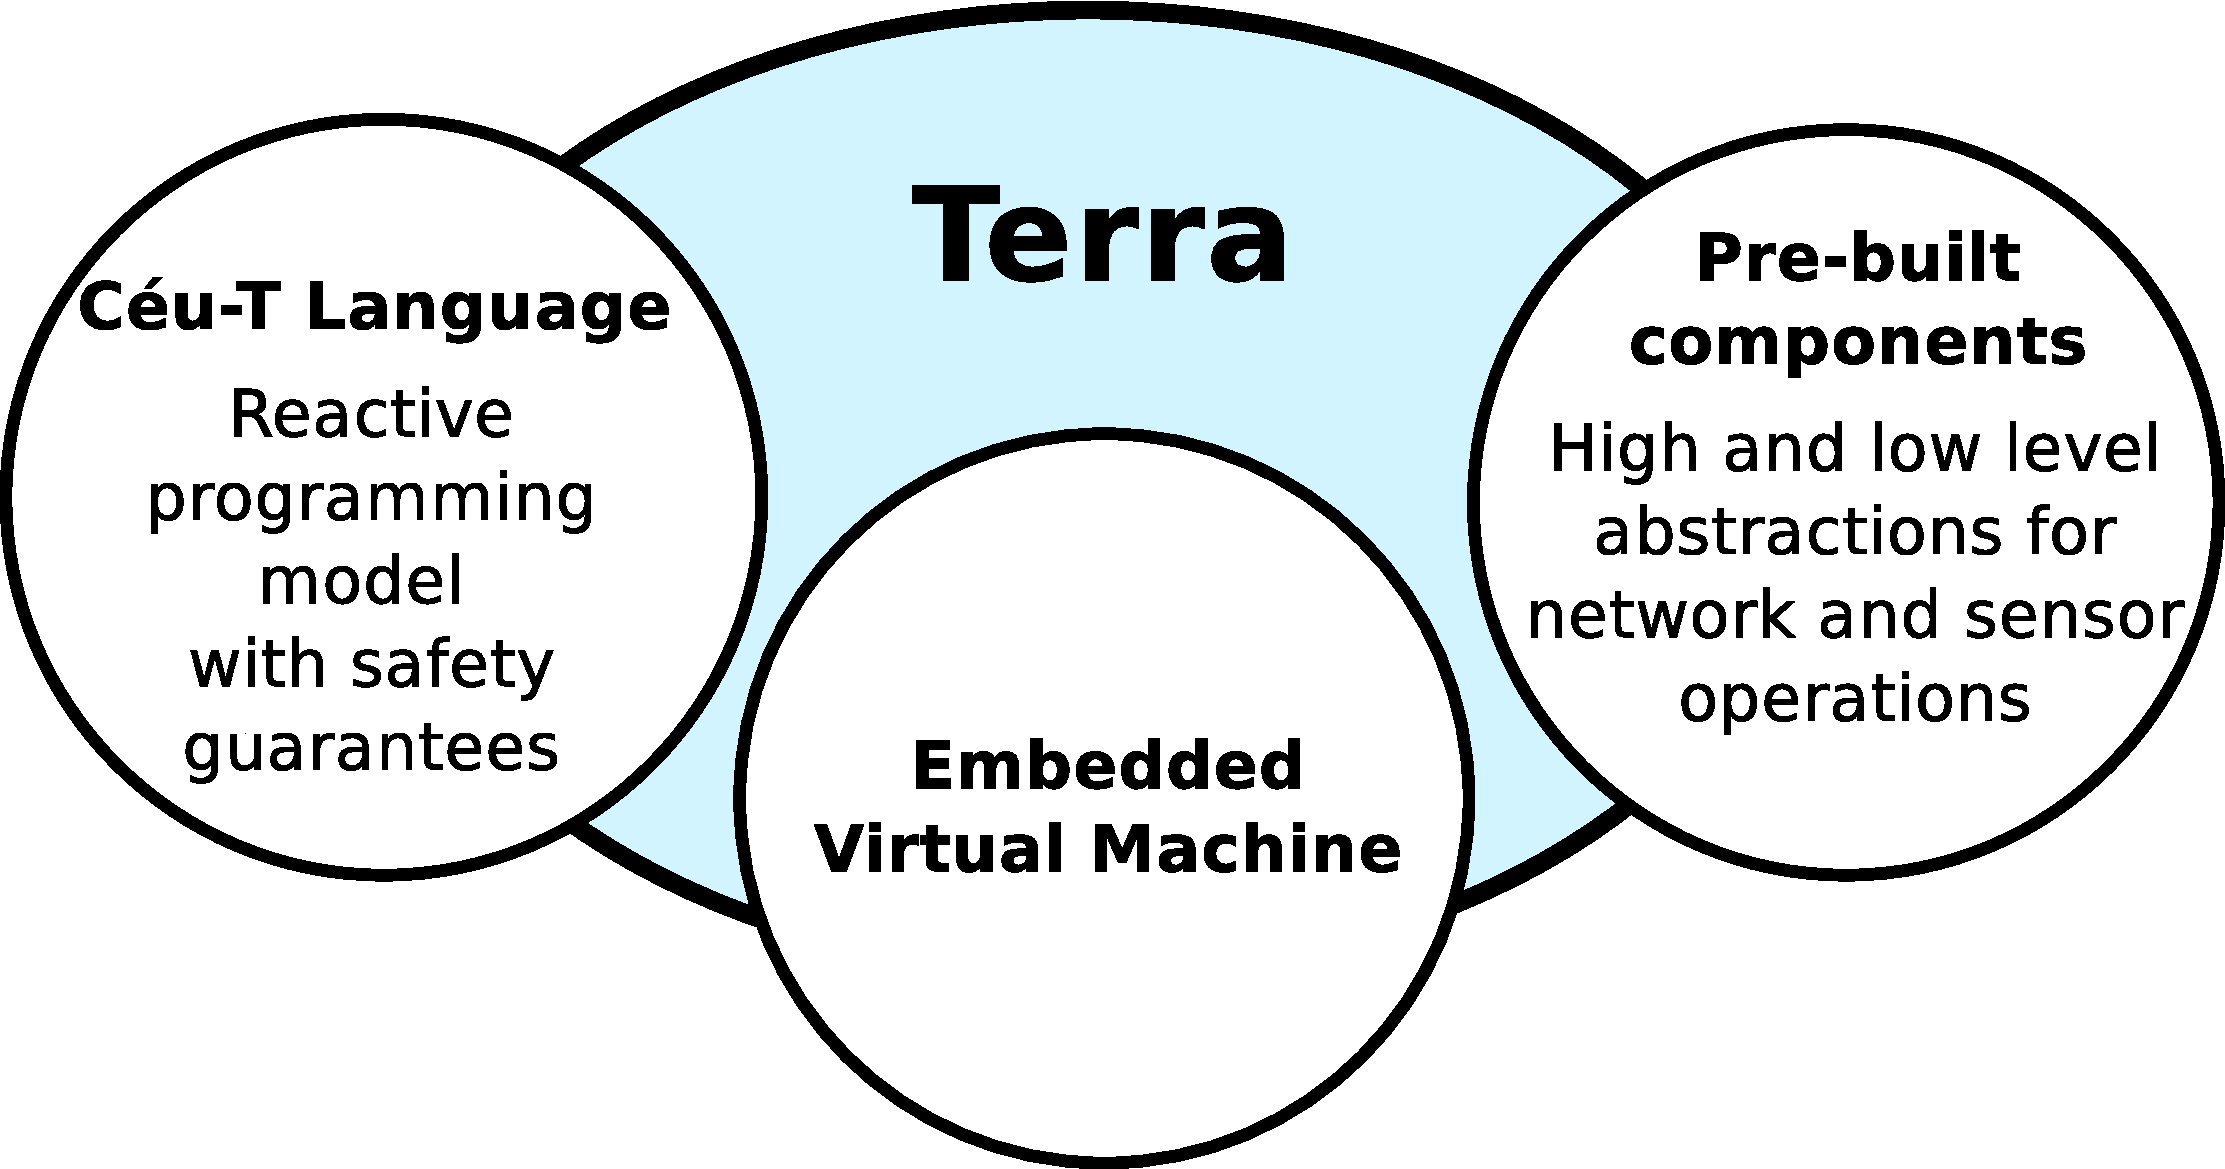
\includegraphics[width=0.5\columnwidth]{terra}
    \caption{Terra programming system basic elements.}
    \label{fig.terra}
\end{figure}

The main difference between the standard \C back end and the Terra \VM is the 
\emph{code generation phase}, which here outputs assembly instructions for the 
\VM (instead of statements in \C).
%
To reduce the memory footprint of applications, the \VM includes special 
instructions for complex and recurrent operations from the runtime of \CEU, 
such as for handling events and trails.

In Terra, \CEU scripts cannot execute arbitrary \C code, instead, they rely on 
pre-built components that can be customized for different application domains.
%
In the domain of sensor networks, Terra already provides components 
organized in four areas: radio communication, group management, data 
aggregation, and local operations (e.g., access to sensors and actuators).
%
When creating an instance of the \VM, the programmer can choose whether or not 
to include each component, setting different abstraction boundaries for 
scripts.
%
The generated \VM has to be preloaded into the embedded devices before they are 
physically distributed.

The communication between scripts in \CEU and the components in the \VM is 
mostly through events:
scripts \code{emit} requests through \code{output} events and \code{await} 
answers through \code{input} events.
%
Terra also provides system calls for initialization and configuration of 
components (e.g., \emph{getters} and \emph{setters}).
%
Figure~\ref{lst.terra.defs}.a shows a \CEU interface with the available 
functionality for a customized \VM (with temperature and radio components).
Figure~\ref{lst.terra.defs}.b shows the associated bindings for output events 
(ln. 1--8), input events (ln. 10--14), and system calls (ln. 16--22).
%
Note that all applications for the customized \VM must comply with the same 
interface.
In contrast, the template-based \C back end (illustrated in 
Figure~\ref{lst.impl.tinyos}) allows applications to choose all possible 
combinations of functionalities from the underlying platform at compile time.

\begin{figure}
\begin{minipage}[t]{0.51\linewidth}
\begin{lstlisting}[morekeywords={function}]
// Output events
output void REQUEST_TEMPERATURE;
output int  REQUEST_SEND;    // sends int value

// Input events
input int  TEMPERATURE_DONE; // recvs int value
input void SEND_DONE;

// System calls
function int getRadioID (void);











.
\end{lstlisting}
\centering\small{\ax}
\end{minipage}
%
\begin{minipage}[t]{0.49\linewidth}
\begin{lstlisting}[numbers=left,xleftmargin=2.5em]
// Output events
void VM.out(int evt_id, void* args) {
    switch (id){
        case O_REQUEST_TEMPERATURE:
            call TINYOS_TEMP.read();
        <...>; // O_REQUEST_SEND
    }
}

// Input events
event TINYOS_TEMP.done (int val) {
    VM.enqueue(I_TEMPERATURE_DONE, &val);
}
<...> // TINYOS_SEND.done

// System calls
void VM.function(int id, void* params) {
    switch (id) {
        case F_GET_RADIO_ID:
            VM.push(TINYOS_NODE_ID);
    }
}
\end{lstlisting}
\centering\small{\bx}
\end{minipage}
%
\caption{
%{\small %\textmd{
\ax \CEU interface with customized \VM.
%
\bx The routine \code{VM.out} redirects all output events to the corresponding 
OS calls (ln.  1--8).
%
Each \emph{TinyOS} event callback calls \code{VM.enqueue} for the corresponding 
input event (ln 10--14).
%
System calls use \code{VM.push} for immediate return values (ln. 16--22).
%
\label{lst.terra.defs}
}
\end{figure}

\section{Related Work}
\label{sec.related}

%\subsection{Semantics}

\CEU has a strong influence from Esterel but differ in the most fundamental 
aspect of the notion of time.
%
In \CEU, instead of clock ticks, atomic external event occurrences that define 
time units.
%
The event-driven approach of \CEU is widespread~\cite{sync_async.whynotthreads} 
and popular in many software communities, such as web frameworks (e.g., 
\emph{jQuery}~\cite{js.jquery} and \emph{Node.js}~\cite{js.node}), GUI toolkits 
(e.g., \emph{Tcl/Tk}~\cite{tcl.tk} and \emph{Java Swing}~\cite{java.swing}), 
and Games~\cite{gamepatterns}.
%
\CEU encrusts this event-triggered notion of time in the core of the language,
which is a prerequisite for the concurrency checks that enable safe
shared-memory concurrency.

In \CEU, internal events support stack-based micro reactions within external
reactions, providing more fine-grained control for intra-reaction execution.
%
Some variants of Statecharts also distinguish internal from external
events~\cite{statecharts.variants}.
%Some variants of Statecharts support local events which imply handling intra
%reactions like \CEU.
In Statemate, \emph{``reactions to external and internal events (...) can be
sensed only after completion of the step''}~\cite{statecharts.statemate},
implying queue-based execution.
In Stateflow, \emph{``the receiving state (of the event) acts here as a
function''}~\cite{statecharts.stateflow}, which is similar to \CEU's
stack-based execution.
To avoid recursion, \CEU adopts delayed awaits, while in Statemate,
\emph{``loops in the broadcasting of events (between states) are forbidden''}.

Like \CEU, many synchronous languages rely on deterministic scheduling to 
preserve intra-reaction determinism (%
\emph{Reactive C}~\cite{rp.rc},                 % 1991
\emph{Protothreads}~\cite{wsn.protothreads},    % 2006
\emph{SOL}~\cite{wsn.sol},                      % 2007
\emph{SC}~\cite{rp.synchc},                     % 2009
and
\emph{PRET-C}~\cite{rp.pretc}).                 % 2010
%
%It is the responsibility of the programmer to specify the execution order for 
%threads, based on either explicit priorities, or source code lexical order 
%(similar to \CEU).
%
In addition, \CEU also performs concurrency checks to detect trails that, when
reordered, change the observable behavior of the program, i.e., trails that
actually rely on deterministic scheduling.
%
%These languages have a tick-based notion of time similar to Esterel, which 
%prevents the concurrency checks of \CEU.
\emph{SCCharts}~\cite{sccharts.1} proposes \emph{sequentially constructive
programs} that allow \emph{``shared variables to have multiple values per tick
as long as these values are explicitly ordered by sequential
statements''}~\cite{sccharts.2}.
This relaxes Esterel's restriction for \emph{read-after-write} accesses only
(e.g., a signal must be emitted to be present) and permits
\emph{write-after-read} accesses typical in imperative programs (e.g., test and
set).
Although this approach still restricts concurrent accesses, it does not impose
strict deterministic scheduling like in \CEU.

\emph{Esterel+Delay}~\cite{esterel.delays} is a non-intrusive extension to
Esterel to program in terms of physical time with \code{delay} statements.
The global transformation relies on a special platform statement the describes
the available timers in the system (e.g., sample-driven or interrupt-driven).
It then expands \code{delay} statements into existing Esterel statements in a
way that the desired semantics can be realised in the platform.
%
\CEU makes physical time a special input event that feeds the runtime with an
associated time to elapse, which is decremented from all awaiting trails.
The compensation scheme of \CEU guarantees that trails awake in the correct
order and that errors are not propagated on subsequent awaits.
Interrupt-driven timers are also supported with a hook callback that the
runtime calls whenever the program awaits an earlier timer.

Regarding resource management, Esterel supports a finalization mechanism to 
unconditionally execute a series of statements on abortion.
%
In addition, \CEU also tracks pointers representing resources that cross \C 
boundaries and forces the programmer to provide associated finalizers.

ReactiveML~\cite{rml} and \emph{URBI}~\cite{rp.urbi} extend the synchronous 
model with dynamic lines of execution.
%
The implementations use coroutines or CPS transformations and rely on heap 
allocation and/or garbage collection, diverging from our goals regarding 
resource efficiency and static bounds for memory and execution time.
%
%These languages and may not be suitable for constrained embedded systems.
%
We discuss dynamic abstractions in \CEU in previous work~\cite{ceu.mod15}.

%\subsection{Implementation}

Esterel has different compilation back ends that synthesizes to software and 
also to hardware circuits~\cite{esterel.emperor,esterel.tutorial}.
Among the software-based approaches,
\emph{SAXO--RT}~\cite{esterel.saxort,esterel.efficient} is the closest to our
implementation with respect to trail allocation and scheduling:
the compiler slices programs into ``control points'' (analogous to our ``entry 
points'') and rearranges them into a directed acyclic graph.
Then, it flattens the graph into sequential code in \C suitable for static 
scheduling.
Esterel compilation is more sophisticated since it involves solving data
dependency relations to comply with its constructive semantics.

%\subsection{VM}

A number of virtual machines have been proposed for embedded systems.
%
%The \emph{Sun SPOT} platform with the \emph{Squawk JVM} brings Java for the 
%embedded domain~\cite{wsn.sunspot}, but requires a much powerful hardware.%
%\footnote{The \emph{Sun SPOT} uses a 32-bit CPU with 4 Mbytes of FLASH and 512 
%KBytes of SRAM.}
%
\emph{Darjeeling}~\cite{wsn.darjeeling} and \emph{TakaTuka}~\cite{wsn.takatuka} 
are complete \emph{Java VMs} targeting constrained embedded systems with 
support for multithreading and garbage collection.
%
Java has antagonistic design choices in comparison to \CEU:
it does not impose static bounds on memory usage and execution time, and 
provides preemptive multithreading which requires synchronization primitives 
for accessing shared memory.
%
An existing Esterel-based VM~\cite{esterel.vm} makes similar design choices to
our work.
To reduce code size, the \VM has a specialized instruction set to deal with 
events and concurrency constructs that are particular to Esterel.
The proposed \VM is only a proof of concept, with no support for 
arithmetic operations, external system calls, or remote reprogramming.

\section{Conclusion}
\label{sec.conclusion}

We present the design and implementation of \CEU, a synchronous reactive 
language inspired by Esterel with event-driven semantics and fine-grained 
control for intra-reaction execution.
%
On the one hand, this approach is familiar to programmers in general,
abstracting tick sampling with reactions to unique events from their
application domain.
On the other hand, this level of abstraction does not suit systems with
hard-real time requirements in which interacting directly with a concrete
notion of tick is more robust.

\CEU is a concurrency-safe language, employing static checks to ensure that 
the high degree of concurrency in embedded systems does not pose safety threats 
to applications.
%
As a summary, the following safety properties hold for all programs that 
successfully compile in \CEU:
time and memory-bounded reactions to the environment (except for system calls),
no race conditions in shared memory,
reliable abortion for activities handling resources,
and automatic synchronization for timers.
%
These properties are usually desirable in embedded applications and are 
guaranteed by design.

\CEU is a resource-efficient language suitable for constrained embedded 
systems.
The reference implementation compiles to portable event-driven code in \C, with 
no special requirements for OS threads or per-trail data stacks.
The \VM implementation uses the same front end and imposes no semantic 
restrictions, being equally suitable for constrained systems.

\CEU is a practical language with expressive control constructs, such as 
lexically scoped parallel compositions, convenient first-class timers, and a 
stack-based mechanism for internal signalling.
%
Programs interoperate seamlessly with \C, and can take advantage of existing 
libraries, lowering the entry barrier for adoption.
%
\CEU has an open source implementation and bindings for \emph{TinyOS}, 
\emph{Arduino}, and the \emph{SDL} graphical library.%
\footnote{Website of \CEU: \url{http://www.ceu-lang.org/}}

For the past three years, we have been teaching \CEU to undergraduate and 
graduate students in courses on \emph{distributed systems} and \emph{reactive 
programming}.
%, in which the students designing protocols, embedded systems, and graphical 
%applications.
%
Our experience shows that students take advantage of the sequential-imperative 
style of \CEU and can implement non-trivial concurrent applications in a few 
weeks.
%
More recently, a company specialized in embedded systems (not related to our 
research group) released a product based on \CEU.

% Bibliography
\bibliographystyle{ACM-Reference-Format-Journals}
\bibliography{my,other,terra}
                             % Sample .bib file with references that match those in
                             % the 'Specifications Document (V1.5)' as well containing
                             % 'legacy' bibs and bibs with 'alternate codings'.
                             % Gerry Murray - March 2012

% History dates
%\received{February 2007}{March 2009}{June 2009}

% Electronic Appendix
%\elecappendix

%\medskip

\end{document}
% End of v2-acmsmall-sample.tex (March 2012) - Gerry Murray, ACM
